
%% Based on a TeXnicCenter-Template, which was
%% created by Christoph Börensen
%% and slightly modified by Tino Weinkauf.
%%%%%%%%%%%%%%%%%%%%%%%%%%%%%%%%%%%%%%%%%%%%%%%%%%%%%%%%%%%%%

\documentclass[a4paper,12pt]{article} %scrartcl This is a special class provided by the KOMA script, which does a lot of adjustments to adapt the standard LaTeX classes to european habits, change to [a4paper,12pt,twoside] for doublesided layout


%########################### Preferences #################################


% ******** vmargin settings *********
\usepackage{vmargin} %This give you full control over the used page arae, it maybe not the idea od Latex to do so, but I wanted to reduce to amount of white space on the page
\setpapersize{A4}
\setmargins{3.5cm}%			%linker Rand, left edge
					 {1.5cm}%     %oberer Rand, top edge
           {14.7cm}%		%Textbreite, text width
           {23.42cm}%   %Texthoehe, text hight
           {30pt}%			%Kopfzeilenhöhe, header hight
           {1cm}%   	  %Kopfzeilenabstand, header distance
           {0pt}%				%Fußzeilenhoehe footer hight
           {2cm}%    	  %Fusszeilenabstand, footer distance   
\setlength{\parindent}{0pt}  % keine Einrückung nach Absatz

% ********* Font definiton ************
\usepackage{t1enc} % as usual
\usepackage[latin1]{inputenc} % as usual
\usepackage{times}		
\usepackage{fancyhdr}
\usepackage[table]{xcolor}
\usepackage{longtable}
\usepackage{wallpaper}

% ********* for code listing ************
\usepackage{listings}  
\usepackage{color}
\definecolor{gray}{rgb}{0.4,0.4,0.4}
\definecolor{darkblue}{rgb}{0.0,0.0,0.6}
\definecolor{cyan}{rgb}{0.0,0.6,0.6}

\lstloadlanguages{XML}

%\lstdefinelanguage{XML}
%{
  %morestring=[b]",
  %morestring=[s]{>}{<},
%%  morecomment=[s]{<?}{?>},
  %morecomment=[s][\color{orange}]{<!--}{-->},
  %stringstyle=\color{black},
  %identifierstyle=\color{darkblue},
  %keywordstyle=\color{red},
  %morekeywords={xmlns,version,type,num},
	%showstringspaces=false,
%}


%\usepackage{mathptmx}  	%mathematical fonts for use with times, I encountered some problems using this package togather with pdftex, which I was not able to resolve

% ********* Graphics definition *******
\usepackage[pdftex]{graphicx} % required to import graphic files
\usepackage{eso-pic} % these two are required to add the little picture on top of every page
\usepackage{everyshi} % these two are required to add the little picture on top of every page
\renewcommand{\floatpagefraction}{0.7} %default:0.5 allows two big pictures on one page
\usepackage{wrapfig}

%********** Enybeling Hyperlinks *******
\usepackage[pdfborder=000,pdftex=true]{hyperref}% this enables jumping from a reference and table of content in the pdf file to its target

% ********* Table layout **************
\usepackage{booktabs}	  	%design of table, has an excellent documentation
\usepackage{multirow}     % multirows in tables

% ********* Caption Layout ************
\usepackage{ccaption} % allows special formating of the captions
\captionnamefont{\bf\footnotesize\sffamily} % defines the font of the caption name (e.g. Figure: or Table:)
\captiontitlefont{\footnotesize\sffamily} % defines the font of the caption text (same as above, but not bold)
\setlength{\abovecaptionskip}{0mm} %lowers the distace of captions to the figure

\usepackage{scrpage2} %header and footer using the options for the KOMA script
\renewcommand{\headfont}{\footnotesize\sffamily} % font for the header
\renewcommand{\pnumfont}{\footnotesize\sffamily} % font for the pagenumbers

\usepackage{helvet}
\renewcommand{\familydefault}{\sfdefault}

% set colors for links and URLs
\usepackage{hyperref}
\hypersetup{
	colorlinks=true,
	linkcolor=black,
	urlcolor=blue}


%this defines the page style for the first pages: all empty
\renewpagestyle{plain}%
	{(\textwidth,0pt)%
		{\hfill}{\hfill}{\hfill}%
	(\textwidth,0pt)}%
	{(\textwidth,0pt)%	
		{\hfill}{\hfill}{\hfill}%
	(\textwidth,0pt)}

%----------------------------------------------------------------------------------------
%	BEGIN DOCUMENT
%----------------------------------------------------------------------------------------

\pagestyle{plain} % on headers or footers on the first page

\begin{document}

%----------------------------------------------------------------------------------------
%	TITLE PAGE
%----------------------------------------------------------------------------------------
\begin{center}
\ThisCenterWallPaper{0.9}{pics/TitleNew.png}
\end{center}

\newpage

\pagestyle{fancy} % now we want to have headers and footers

%----------------------------------------------------------------------------------------
%	Header and Footer
%----------------------------------------------------------------------------------------
\fancyhf{} %alle Kopf- und Fußzeilenfelder bereinigen
\fancyhead[R]{} %Kopfzeile rechts
\fancyhead[C]{} %zentrierte Kopfzeile
\fancyhead[L]{
\includegraphics[height=30pt]{pics/logosSUM.png}} %Kopfzeile links
\renewcommand{\headrulewidth}{0.4pt} %obere Trennlinie
\fancyfoot[L]{{PRo3D 2.0}} 
\fancyfoot[R]{\thepage} 
\renewcommand{\footrulewidth}{0.4pt} %untere Trennlinie

%----------------------------------------------------------------------------------------
%	Change Records 
%----------------------------------------------------------------------------------------

%\begin{table}[h]
	%\centering
	%
		%\caption{\textbf{Change Records}}
		%\label{tab:changeRecs}
		%
		%\rowcolors{1}{lightgray}{white}
%
		%\begin{tabular}{c c p{7cm} p{3cm}}
			%\textbf{ISSUE} & \textbf{DATE} & \textbf{§ CHANGE RECORDS} & \textbf{AUTHOR} \\
			%\hline
			%1.0 & 2018-01-23 & Initial Version & Ortner, Fritz
		%\end{tabular}
%
%\end{table}

\newpage

%----------------------------------------------------------------------------------------
%	Table of Contents + List of Figures
%----------------------------------------------------------------------------------------
\tableofcontents
%\listoffigures

\newpage
%----------------------------------------------------------------------------------------
%	Section: Introduction
%----------------------------------------------------------------------------------------
%----------------------------------------------------------------------------------------
%	Section: Introduction
%----------------------------------------------------------------------------------------
\section{Introduction}

\begin{figure}[h]
    	\centering
    		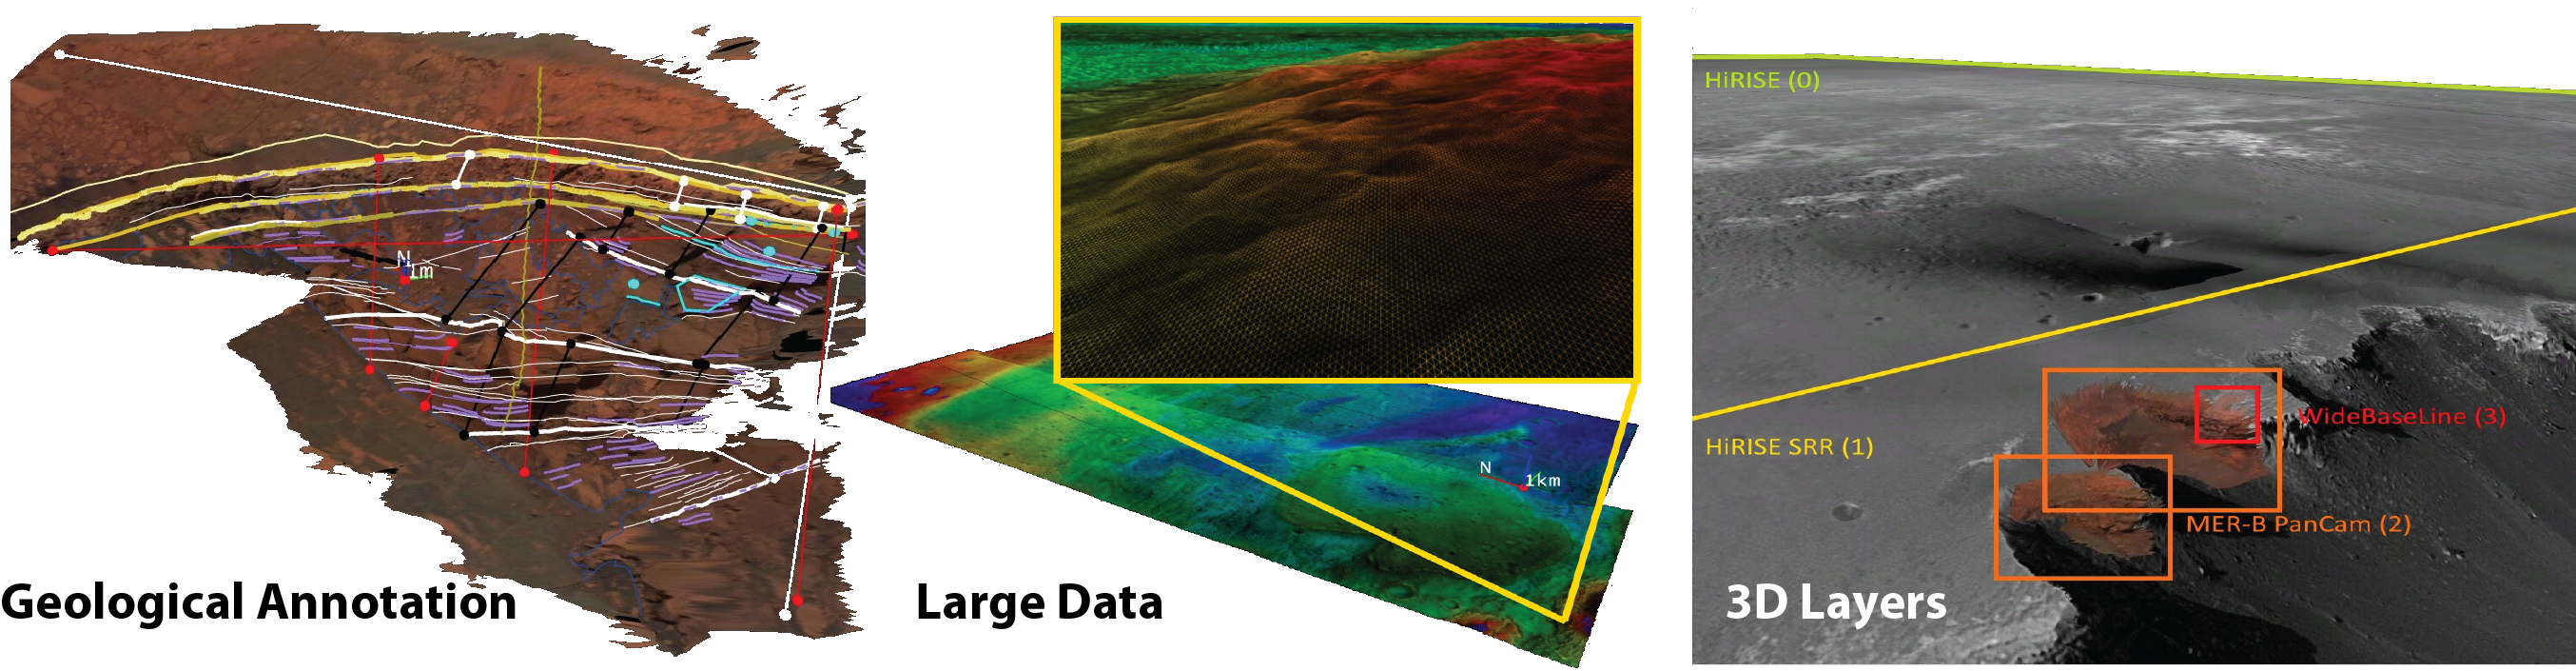
\includegraphics[width=1\textwidth]{pics/Features.png}
    	%\caption[Viewer Features]{}
    	\label{fig:Features}
   \end{figure}
	
PRo3D, short for \textbf{P}lanetary \textbf{Ro}botics \textbf{3D} Viewer, is an interactive 3D visualization tool to allow planetary scientists to work with high-resolution 3D reconstructions of the Martian surface.
%----------------------------------------------------------------------------------------
%	SubSection: Who uses PRo3D
%----------------------------------------------------------------------------------------
\subsection{Who uses PRo3D}
\label{sec:whoUsesP3D}

PRo3D aims to support planetary scientists in the course of NASA's and ESA's missions to find signs of life on the red planet by exploring high-resolution 3D surface reconstructions from orbiter and rover cameras.

For the past 5 years the development of PRo3D has been geared towards providing planetary \textbf{geologists} with interactive tools to digitize geological features on digital outcrop models (DOMs) on the Martian surface. During our fruitful cooperation with geologists from the Imperial College of London, PRo3D has emerged as their main tool to conduct remote geological analysis which lead to many publications and talks at various geological science venues.

Planetary geology is the most elaborately supported use-case of PRo3D, however we strive to expand our user groups to other use-cases, so we have also developed features for supporting science goals in \textbf{landing site selection} and \textbf{mission planningabc}.

%----------------------------------------------------------------------------------------
%	SubSection: Features
%----------------------------------------------------------------------------------------
\subsection{Features}
\label{sec:features}

\begin{itemize}
	\item \textbf{Geological Annotation}: PRo3D lets users pick points on the 3D surface at the full resolution of the data present. Our tools contain point, line, and polyline annotations, while line segments are projected onto the surface. Various measurements are computed at the highest possible accuracy, such as the distance along a 3D surface (waylength) or dip-and-strike orientations of sediment structures. 
	\item \textbf{Large Data}: Surface reconstructions from high-resolution satellite images can easily yield gigabytes of data in terms of geometry, imagery, and additional layers. With PRo3D users can explore huge datasets interactively and even perform measurements of topographic features. The displayed dataset on the right consists of 2GB of raw 3D position vectors, a 1GB elevation map, and 10GB of image data rendered at interactive framerates with commodity hardware, utilizing adjustable level-of-detail and out-of-core techniques. 
	\item \textbf{3D Layers}: Although, PRo3D is not a GIS system, we need to provide our users with typical GIS features to solve their geospatial problems, such as evaluating topographic or geological features. Our 3D layering technique allows a seamless integration of different reconstructions present at a single location. Unlike image or DTM layering we allow users to blend full 3D data by assigning rendering priorities, which is crucial to explore reconstructions from multiple rover camera instruments. 
\end{itemize}
%----------------------------------------------------------------------------------------
%	SubSection: Data
%----------------------------------------------------------------------------------------
\subsection{Data}
\label{sec:data}

Currently, PRo3D only supports reconstructions in the proprietary data format OPC (Ordered Point Clouds), basically consisting of hierarchically organized surface patches. These reconstructions stem from orbiter images and rover images and are produced by Joanneum Research by using the PRoViP processing pipeline. Many surface reconstructions have been generated from, for instance: HiRISE, MER-A, MER-B and MSL missions from various instruments. An ongoing project evaluates terrestrial applicability of PRo3D and the PRoViP pipeline by capturing outcrops in the UK. 


%----------------------------------------------------------------------------------------
%	Section: Start
%----------------------------------------------------------------------------------------
%----------------------------------------------------------------------------------------
%	Section: Start
%----------------------------------------------------------------------------------------
\section{Start}

Start the viewer by clicking the PRo3D.exe and open the Scene Menu in the top left of the window shown in Figure~\ref{fig:StartMenu}.
\begin{figure}[h]
    	\centering
    		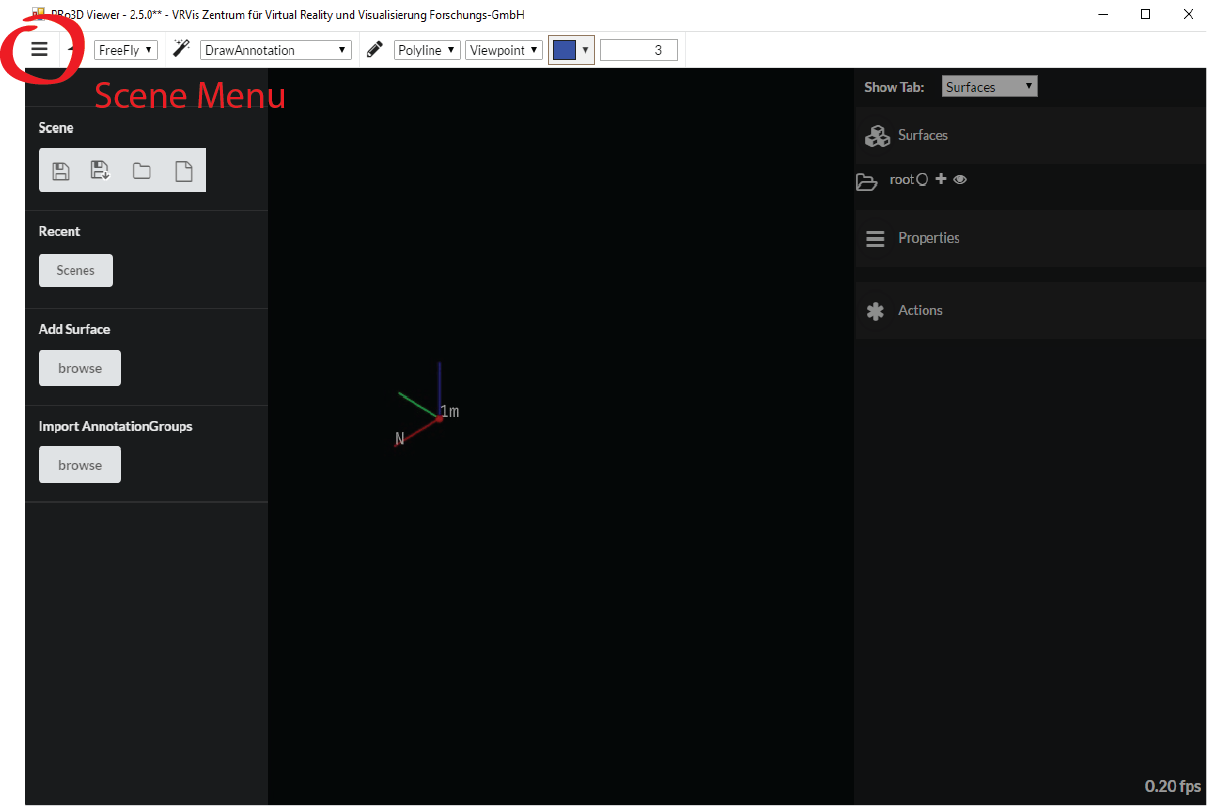
\includegraphics[width=1\textwidth]{pics/startMenuAI.png}
    	\caption[Start Menu]{Open Scene Menu. }
    	\label{fig:StartMenu}
   \end{figure}

You have two options to start:
\begin{itemize}
	\item Add one or more surfaces and create a new scene as described in the next Section~\ref{sec:addSurface}.
	\item Load an existing scene described in the Section~\ref{sec:loadScene}. 
\end{itemize}


%In the scene menu you have the following sections:
%\begin{itemize}
	%\item \textbf{Scene:}
	%\item \textbf{Recent:}
	%\item \textbf{Add Surface:}
	%\item \textbf{ImportAnnotationGroups:}
%\end{itemize}

%----------------------------------------------------------------------------------------
%	SubSection: Add Surface
%----------------------------------------------------------------------------------------
\subsection{Add Surface}
\label{sec:addSurface}

To add a new surface click the ``Browse'' button in the \textbf{AddSurface} section in the scene menu (Figure~\ref{fig:StartMenu}).
This opens the ``Select Folder'' window where you can choose the surface folder as shown in Figure~\ref{fig:AddSurface}. Click the ``Select Folder'' button to confirm your selection. The surface is loaded into the viewer and listed in the right part of the window as shown in Figure~\ref{fig:NewSurface}, part A.
You can add more surfaces in the same way.
	
	\begin{figure}[h]
    	\centering
    		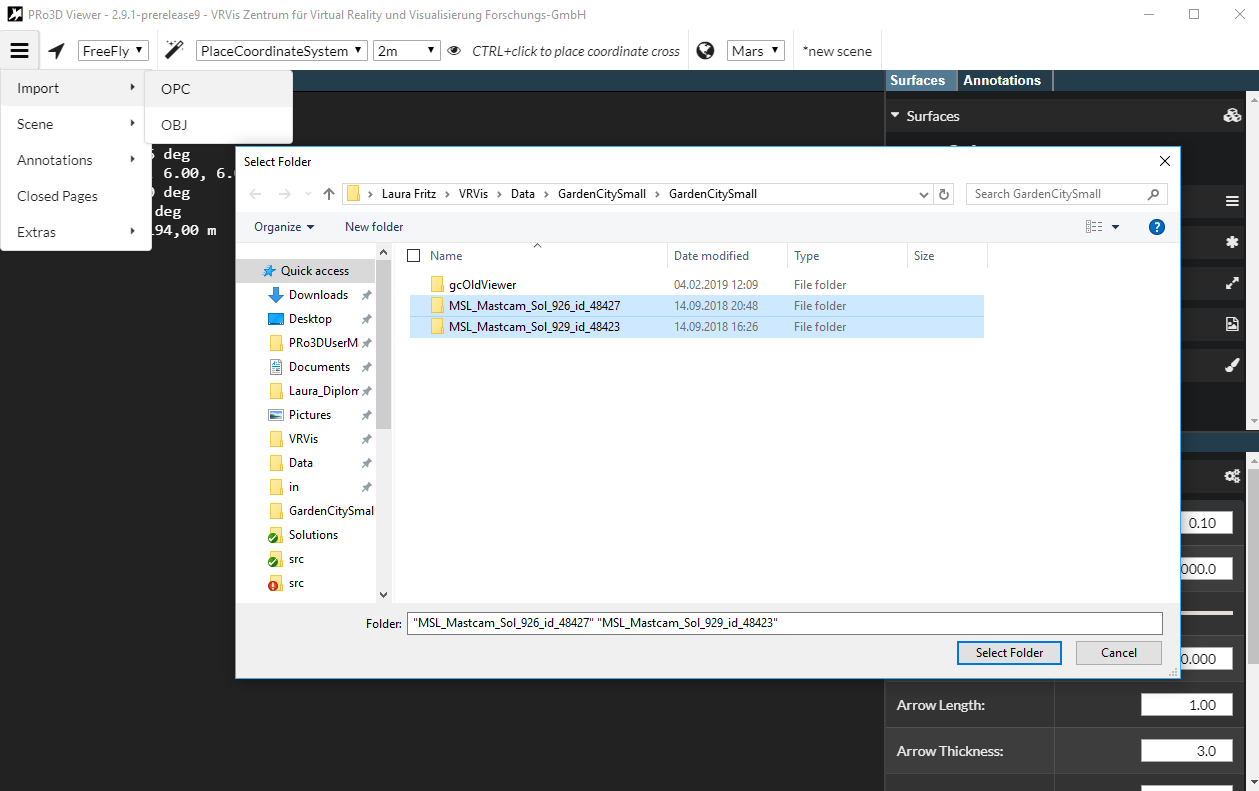
\includegraphics[width=1\textwidth]{pics/AddSurface.png}
    	\caption[Add Surface]{Add a new surface to the scene.}
    	\label{fig:AddSurface}
   \end{figure}
	
	
Each surface has a little context menu below the surface's name in the list (Figure~\ref{fig:NewSurface}, B). Click the ``FlyTo'' button to see the surface in the main window. To see the surface's properties click on the appropriate name in the list (Figure~\ref{fig:NewSurface}, C).
	
Finally, click ``SaveScene'' in the scene menu, name the scene and press the ``Save'' button (Figure~\ref{fig:saveScene}) to save the surfaces and your settings. The PRo3D viewer will load the scene automatically next time you start the viewer.
	
	\begin{figure}[h]
    	\centering
    		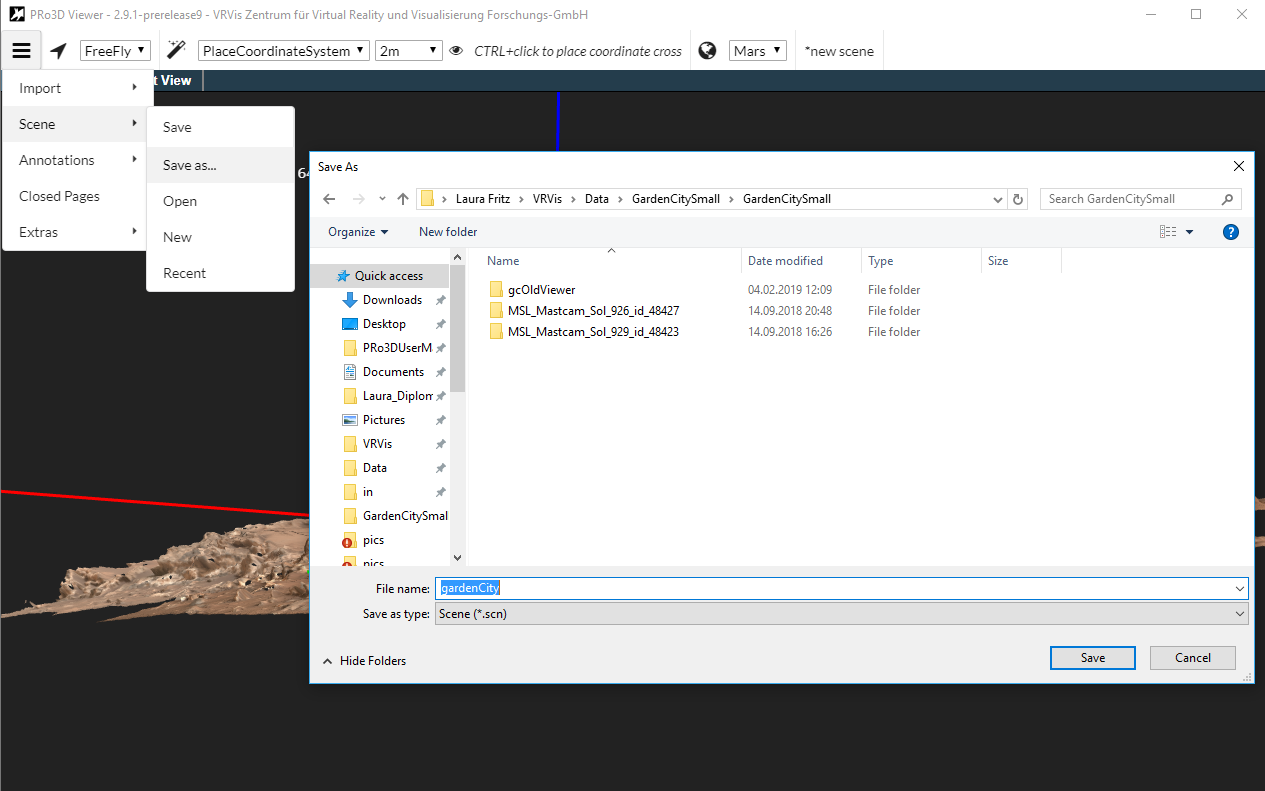
\includegraphics[width=1\textwidth]{pics/saveScene.png}
    	\caption[Save Scene]{Save the surfaces and settings as scene. }
    	\label{fig:saveScene}
   \end{figure}
		
%----------------------------------------------------------------------------------------
%	SubSection: Load Scene
%----------------------------------------------------------------------------------------
\subsection{Load Scene}
\label{sec:loadScene}

Load an existing scene by selecting ``Open Scene'' in the \textbf{Scene} section in the start menu (Figure~\ref{fig:StartMenu}).
Select the scene xml file in the directory of your choice and confirm your selection (Figure~\ref{fig:OpenScene}).
Then the scene is loaded (Figure~\ref{fig:NewSurface}). 

\begin{figure}[h]
    	\centering
    		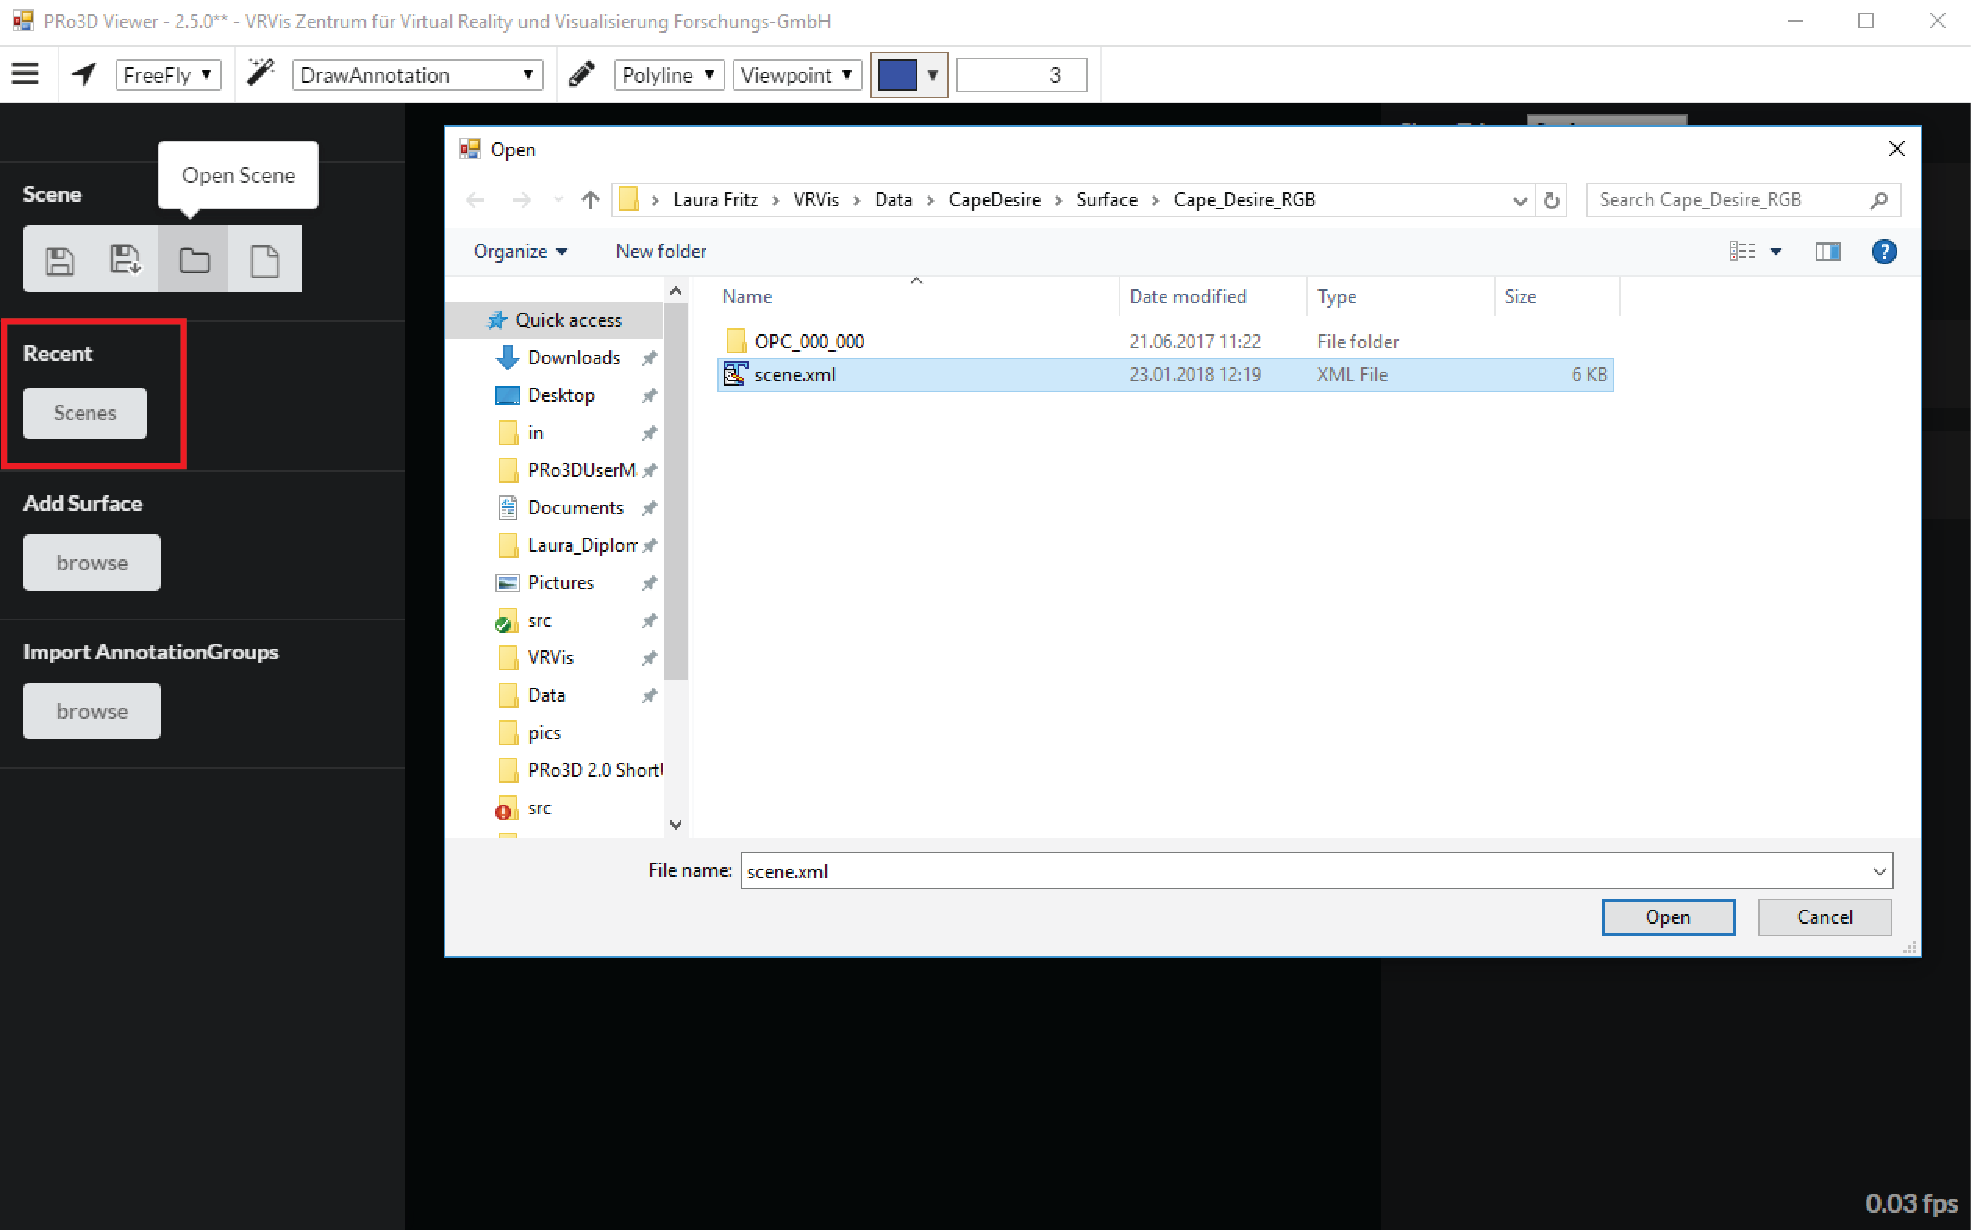
\includegraphics[width=1\textwidth]{pics/OpenSceneAI.png}
    	\caption[Open Scene]{ Open a scene with either the ``Open Scene'' button in the scene section, or with the ``Scenes'' button in the recent section (red rectangle).}
    	\label{fig:OpenScene}
   \end{figure}
	
You can also load recent scene files with the ``Scenes'' button in the \textbf{Recent} section (red rectangle in Figure~\ref{fig:OpenScene}). By hovering with the mouse over the button,
a tool tip menu with a list of recent scenes opens. Click on the required scene name to load the scene.

\begin{figure}[h]
    	\centering
    		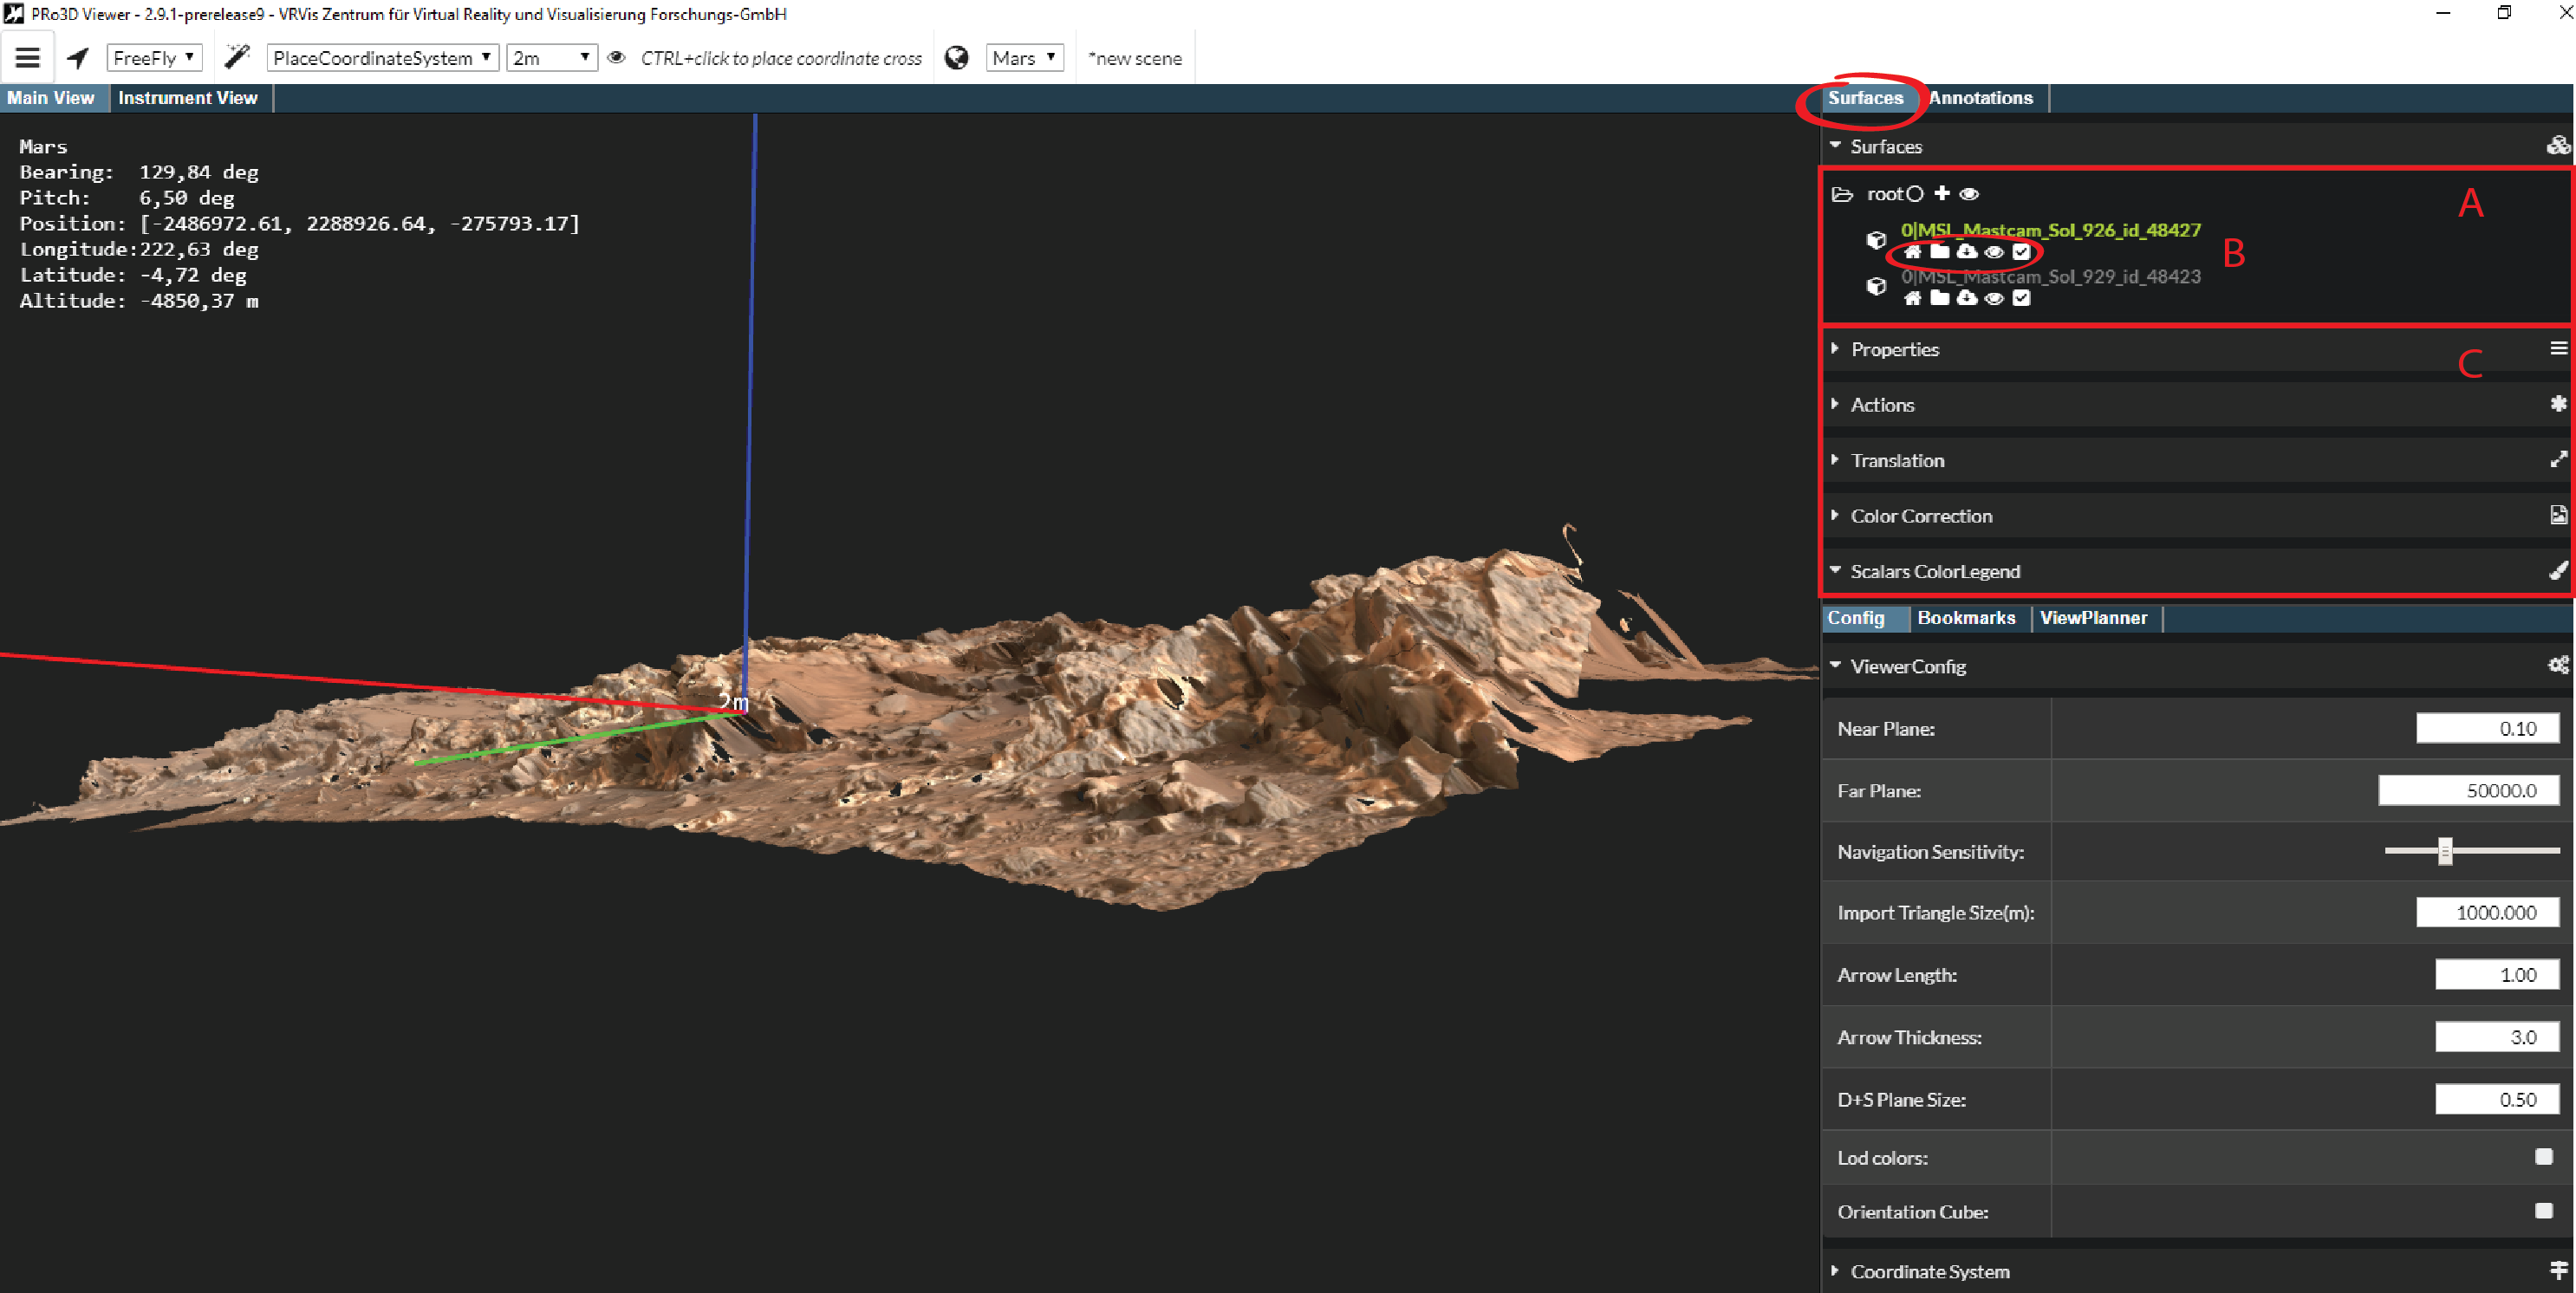
\includegraphics[width=1\textwidth]{pics/NewSurfaceAI.png}
    	\caption[New Surface]{Loaded surface with open surface features (right).}
    	\label{fig:NewSurface}
   \end{figure} 
	
%----------------------------------------------------------------------------------------
%	Section: Viewer Actions
%----------------------------------------------------------------------------------------
%----------------------------------------------------------------------------------------
%	Section: Viewer Actions
%----------------------------------------------------------------------------------------
\section{Viewer Actions}

\begin{figure}[h]
    	\centering
    		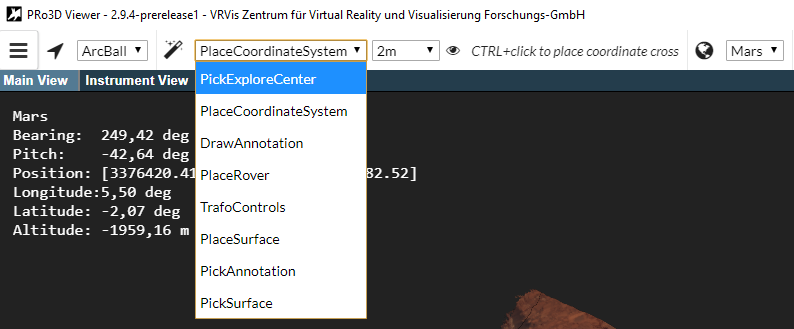
\includegraphics[width=1\textwidth]{pics/Interactions.png}
    	\caption[Interactions]{Viewer Actions.}
    	\label{fig:Interactions}
   \end{figure}

Once the surface is loaded there are different actions to choose (Figure~\ref{fig:Interactions}).
%----------------------------------------------------------------------------------------
%	SubSection: Pick Explore Center
%----------------------------------------------------------------------------------------
\subsection{Pick Explore Center}
\label{sec:pickEC}

The ``PickExploreCenter'' action concerns the \textbf{ArcBall} navigation mode. There are two navigation modes (Figure~\ref{fig:exploreCenter}):
\begin{itemize}
	\item \textbf{FreeFly} and 
	\item \textbf{ArcBall}.
\end{itemize}

\begin{figure}[h]
    	\centering
    		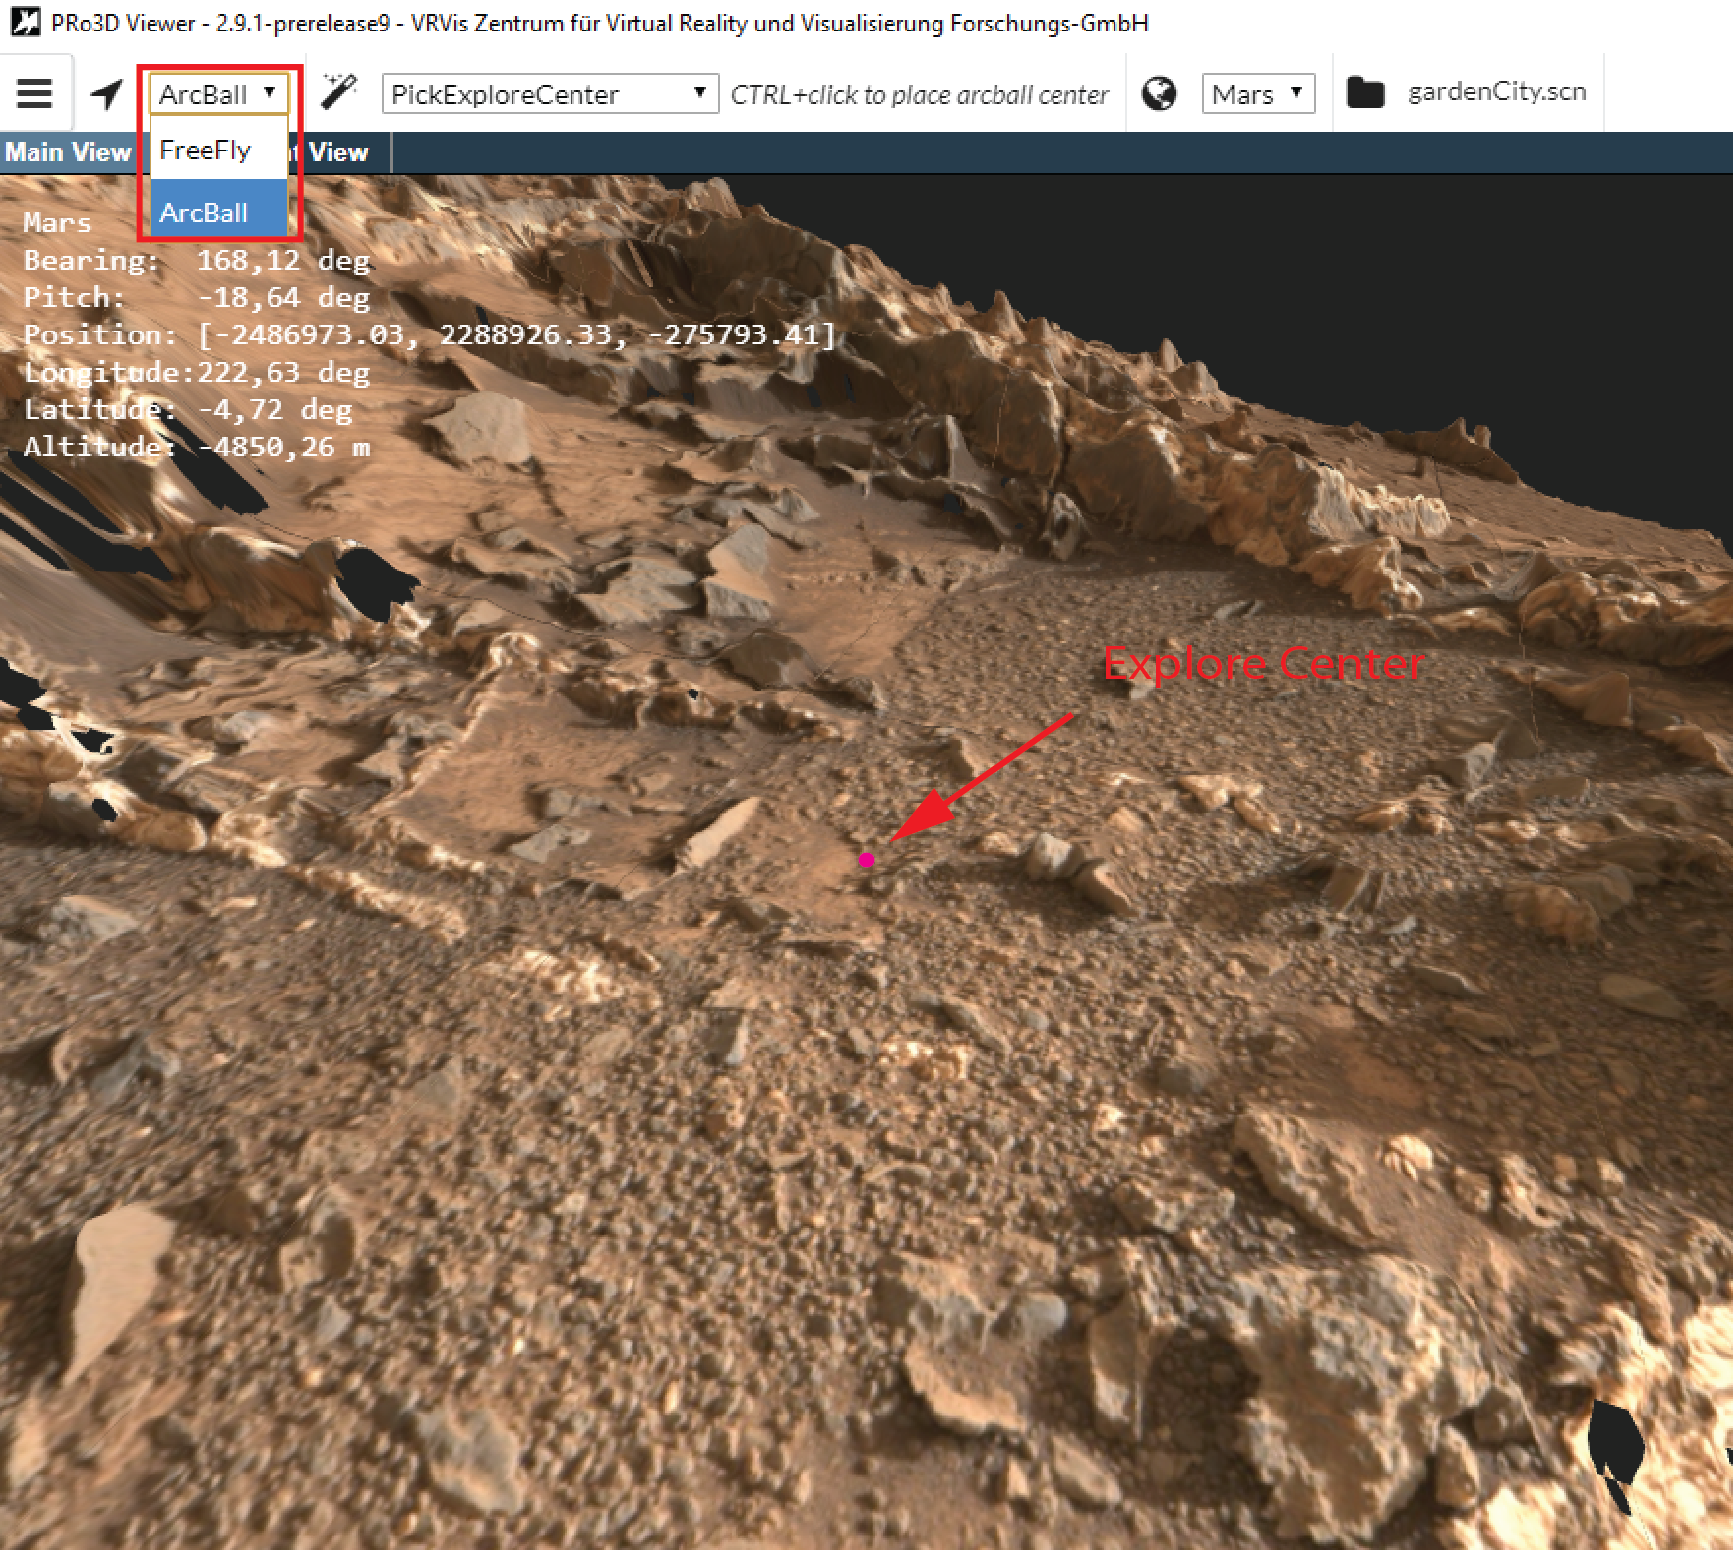
\includegraphics[width=1\textwidth]{pics/exploreCenterAI.png}
    	\caption[ExploreCenter]{ArcBall navigation. Explore center is set with CTRL + LMB and indicated by a pink dot.}
    	\label{fig:exploreCenter}
   \end{figure}

%----------------------------------------------------------------------------------------Free Fly-
\subsubsection{FreeFly}

The Free Fly Mode is the standard 3D fly-through navigation, as for instance, in terrain visualization. WASD controls forward/backward and strafing movement, while the user can change the camera's orientation by holding the LMB (= \textbf{L}eft \textbf{M}ouse \textbf{B}utton). Zooming in and out (forward/backward movement) is performed by turning the mouse-wheel or holding down the RMB (= \textbf{R}ight \textbf{M}ouse \textbf{B}utton). Additionally, the camera can be panned by holding down the middle mouse button.

%----------------------------------------------------------------------------------------Arc Ball-
\subsubsection{ArcBall}

When the viewer is in ArcBall mode the camera can be rotated around the explore center by holding down the LMB. Panning and strafing as possible as described above, but be aware that this moves the explore center (otherwise panning would break the view matrix of the camera). To set a new explore point, make sure the ``PicExploreCenter'' action is active (as shown in Figure~\ref{fig:exploreCenter}) and press CTRL + LMB on the surface. The explore center is indicated by a pink dot. Forward and backward movement is performed either by the keys W/S, rotating the mouse wheel, or clicking RMB.
%----------------------------------------------------------------------------------------
%	SubSection: Place Coordinate System
%----------------------------------------------------------------------------------------
\subsection{Place Coordinate System}
\label{sec:placeCS}

\begin{figure}[h]
    	\centering
    		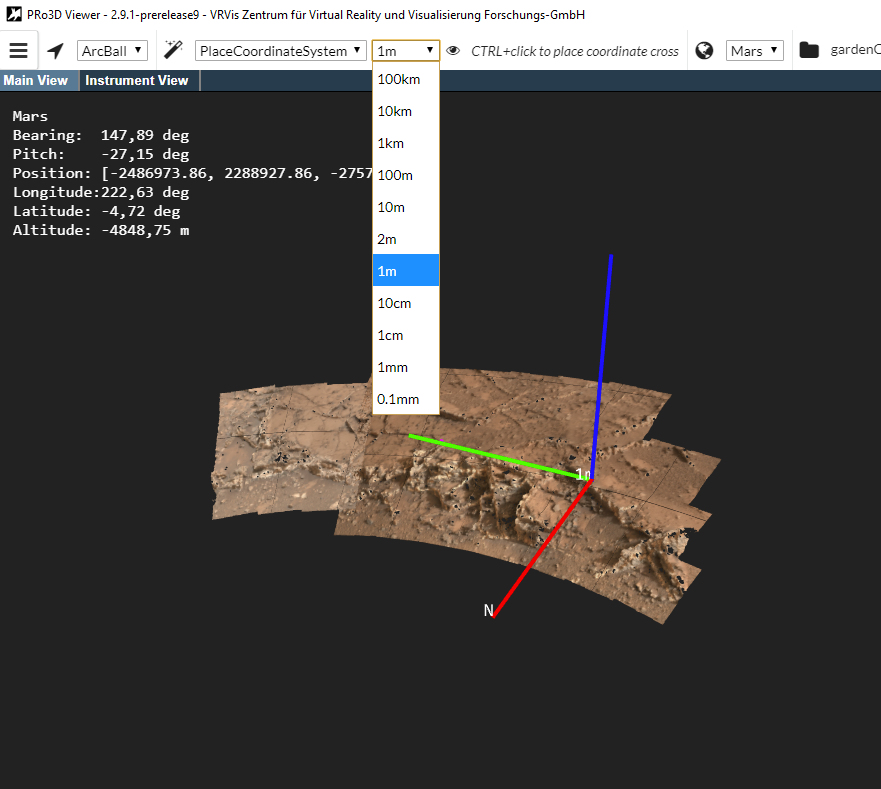
\includegraphics[width=1\textwidth]{pics/CoordinateSystem.png}
    	\caption[Coordinate System]{Coordinate System with scale bar functionality.}
    	\label{fig:coordinateSystem}
   \end{figure}
	
To set the coordinate system pick ``PlaceCoordinateSystem'' in the actions drop down menu, select a unit of measurement and press CTRL+LMB to pick a point on the surface. This marks the position as shown in Figure~\ref{fig:coordinateSystem}.
Initially the up vector's (blue) direction is set in the positive z-direction and the north vector's (red) in the positive y-direction. You can manipulate the north vector manually for different data. The surface can be translated along the three directions of the coordinate system, as described in Section~\ref{sec:surfaces}. The up- and the north vector are used for the projection measurements. The north vector is further relevant for bearing measurements and the rover placement in the View Planner.
%(see Section~\ref{sec:viewPlanner})
The value for manipulating the north vector is shown in the Viewer Configuration described in Section~\ref{sec:config}.
%----------------------------------------------------------------------------------------
%	SubSection: Draw Annotation
%----------------------------------------------------------------------------------------
\subsection{Draw Annotation}
\label{sec:drawAnnotation}

\begin{figure}[h]
    	\centering
    		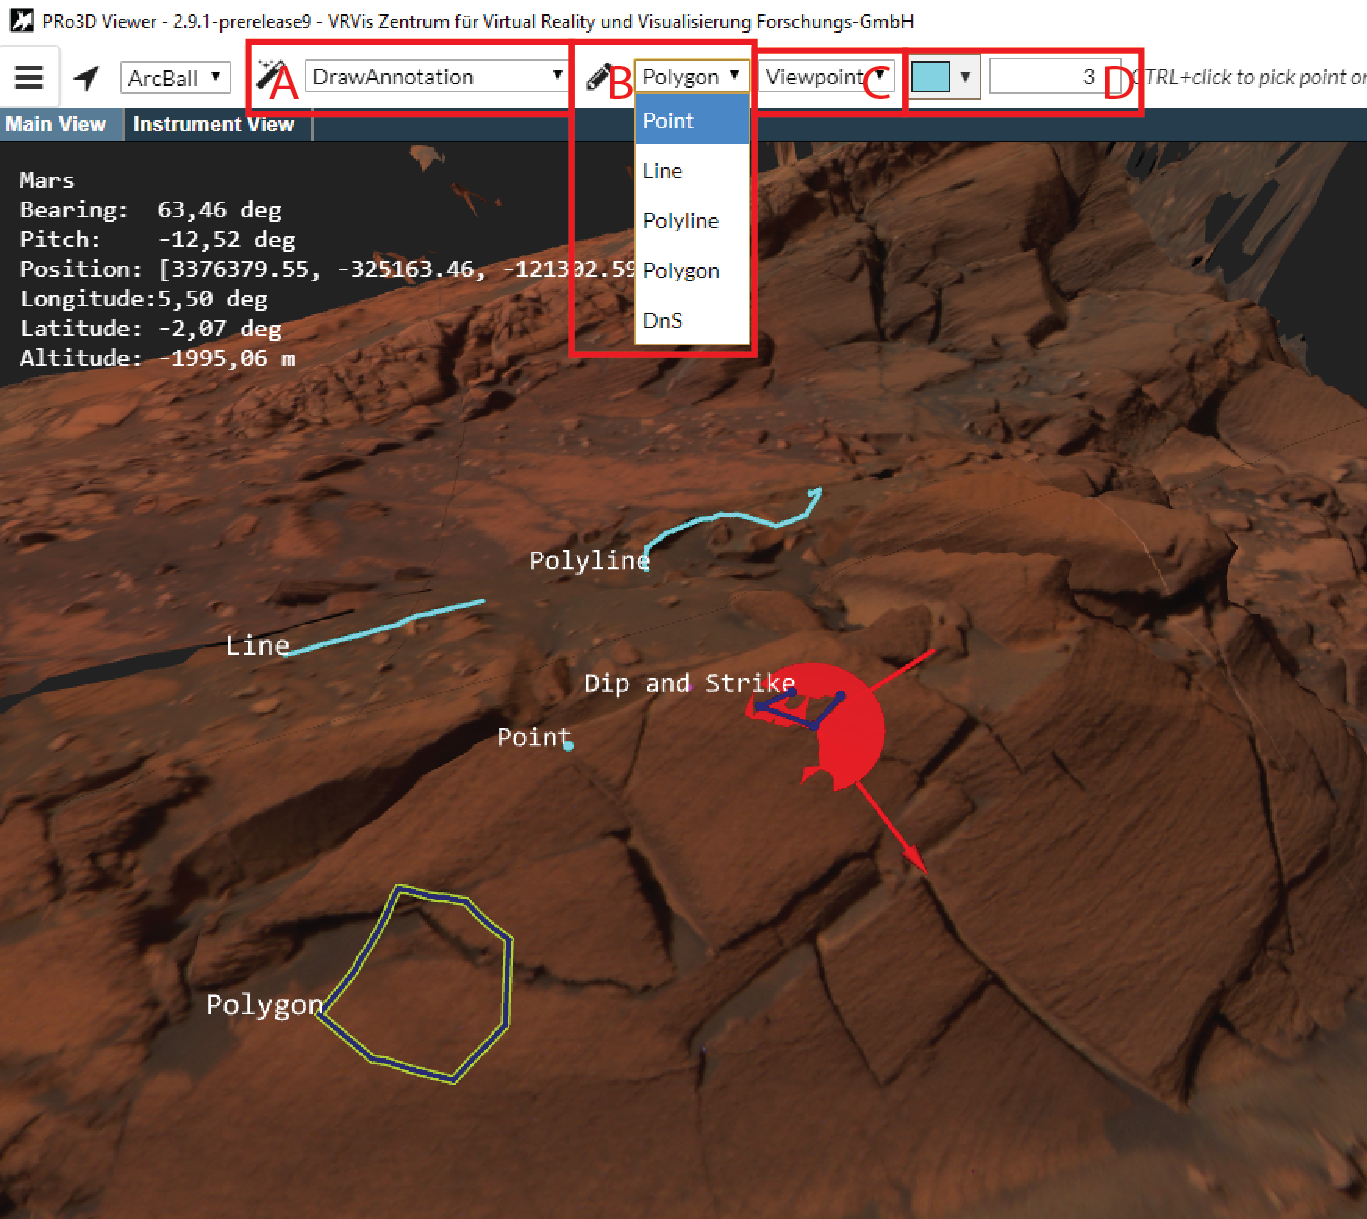
\includegraphics[width=1\textwidth]{pics/drawAnnotationsAI.png}
    	\caption[Draw Annotations]{Annotation settings: \textbf{A}: set viewer action to ``DrawAnnotation. \textbf{B}: select annotation mode. \textbf{C}: select projection. \textbf{D}: choose color and thickness. }
    	\label{fig:drawAnnotations}
   \end{figure}
	
Figure~\ref{fig:drawAnnotations} shows the settings for drawing annotations. First set ``DrawAnnotation'' in the actions menu (A in Figure~\ref{fig:drawAnnotations}). Then you can choose one of the following annotation modes (B in Figure~\ref{fig:drawAnnotations}):
\begin{itemize}
	\item \textit{Point}: A single point measurement on the surface.
	\item \textit{Line}: You can pick two points on the surface. The connecting line depends on the projection mode explained in the table below.
	\item \textit{Polyline}: An arbitrary number of points on the surface can be picked. The connecting line segments depend on the projection mode. The polyline is finished by pressing Enter.
	\item \textit{Polygon}: An arbitrary number of points on the surface can be picked. The connecting line segments depend on the projection mode. The region of interest is closed and finished by pressing Enter.
	\item \textit{DnS}: A polyline onto a surface, e.g. alongside a rock layer can be picked. After clicking Enter, a plane is fitted (least squares) to this polyline (blue), which is then intersected with a horizontal plane, which gives us the so-called strike vector (red). This vector represents the direction within the plane with the least inclination and orthogonal to it is the dip vector (green) which shows the direction of highest inclination as shown in Figure~\ref{fig:drawAnnotations}.
\end{itemize}
To pick an annotation point on the surface press CTRL+LMB.

For all annotations (except Point) you can choose between ``Linear'', ``ViewPoint'' and ``Sky'' projection which determines the direction of the picking ray (C in Figure~\ref{fig:drawAnnotations}):
\begin{itemize}
	\item \textit{Linear}: produces straight line segments as point-to-point connections with linear interpolation between them, no actual projection is performed (Figure~\ref{fig:projection}, blue line). This is practical for line-of-flight distance measurements or measuring the height of a cliff or determining its slope.
	\item \textit{ViewPoint}: between two points we sample the space by shooting additional rays to intersect with the surface, in this case along the view direction (Figure~\ref{fig:projection}, green line). This is helpful to measure details in nooks and crannies of a rough surface and is the typical way to go for geological measurements.
	\item \textit{Sky}: the same sampling happens as for the viewpoint projection but this time the rays are shot along the scenes up-vector (Figure~\ref{fig:projection}, pink line). This mode is useful for geographical measurements to estimate the length of a path through a crater.
\end{itemize}

\begin{figure}[h]
    	\centering
    		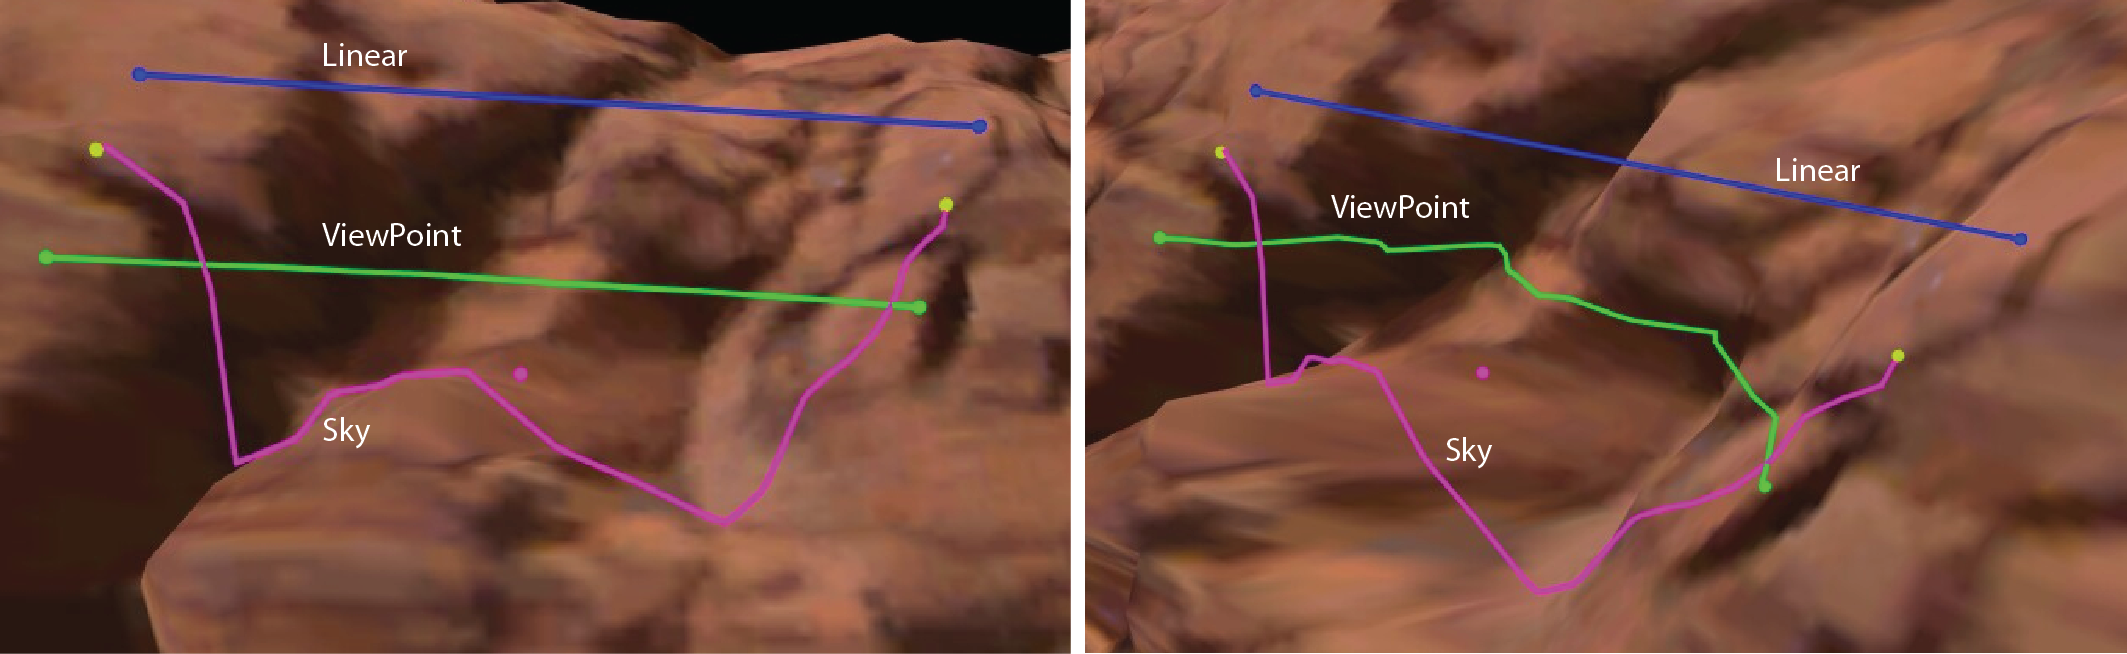
\includegraphics[width=1\textwidth]{pics/projectionAI.png}
    	\caption[Projections]{Three Lines taken from the same camera position (left) with the same camera settings but with different line projections.}
    	\label{fig:projection}
   \end{figure}
	
Finally you can set the color and thickness of the annotation (D in Figure~\ref{fig:drawAnnotations}).
Section~\ref{sec:annotations} shows how to maintain, group and edit existing annotations.
%----------------------------------------------------------------------------------------
%	SubSection: Place Rover
%----------------------------------------------------------------------------------------
%\subsection{Place Rover}
%\label{sec:placeRover}

%----------------------------------------------------------------------------------------
%	SubSection: Trafo Controls
%----------------------------------------------------------------------------------------
%\subsection{Trafo Controls}
%\label{sec:trafoControls}

%----------------------------------------------------------------------------------------
%	SubSection: Align Pick
%----------------------------------------------------------------------------------------
%\subsection{Align Pick}
%\label{sec:alignPick}


%----------------------------------------------------------------------------------------
%	Section: Viewer Features
%----------------------------------------------------------------------------------------
%----------------------------------------------------------------------------------------
%	Section: Viewer Features
%----------------------------------------------------------------------------------------
\section{Viewer Features}

\begin{figure}[h]
    	\centering
    		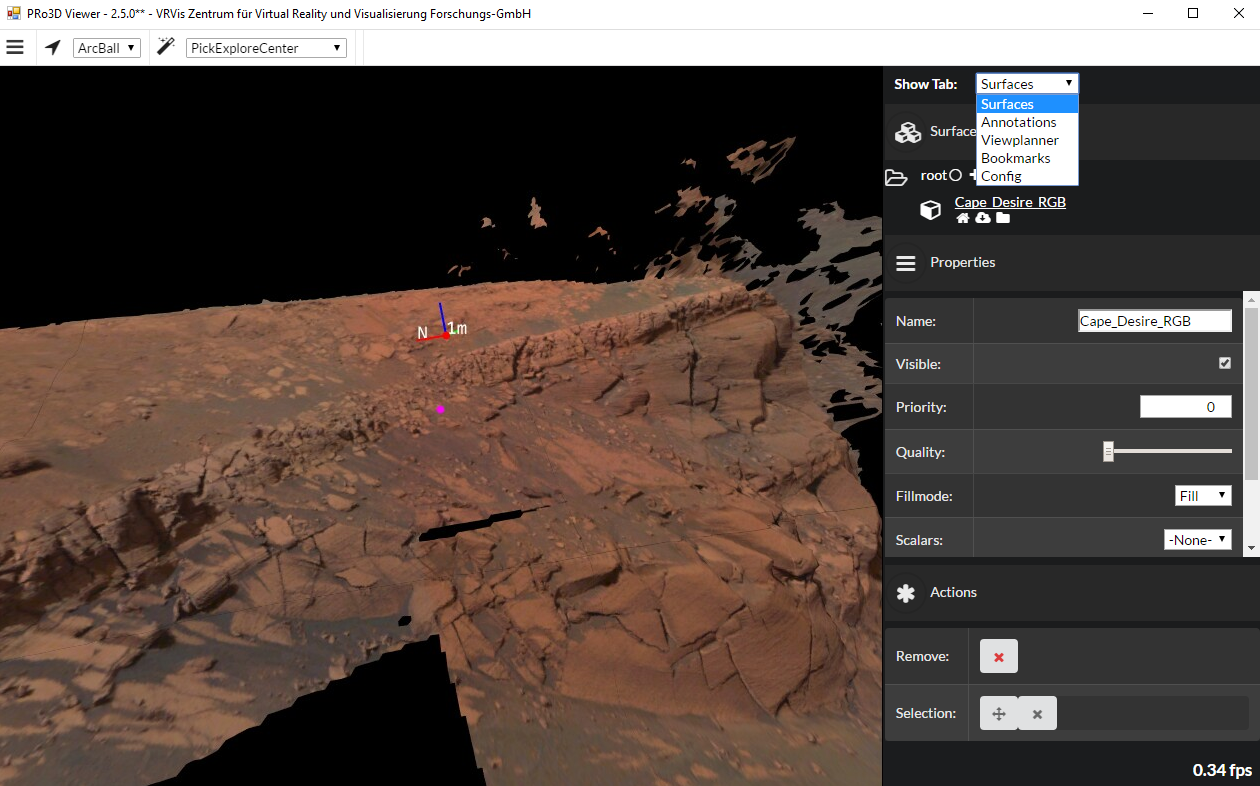
\includegraphics[width=1\textwidth]{pics/featureMenu.png}
    	\caption[Viewer Features]{There are menu tabs (right) for each feature in the viewer.}
    	\label{fig:featureMenu}
   \end{figure}
	
The feature tabs show a list of the respective features, the properties of the selected feature from this list and some actions for this feature.
For surfaces, annotations and bookmarks it is possible to group them, as described in Section~\ref{sec:grouping}.
%----------------------------------------------------------------------------------------
%	SubSection: Surfaces
%----------------------------------------------------------------------------------------
\subsection{Surfaces}
\label{sec:surfaces}

\begin{figure}[h]
    	\centering
    		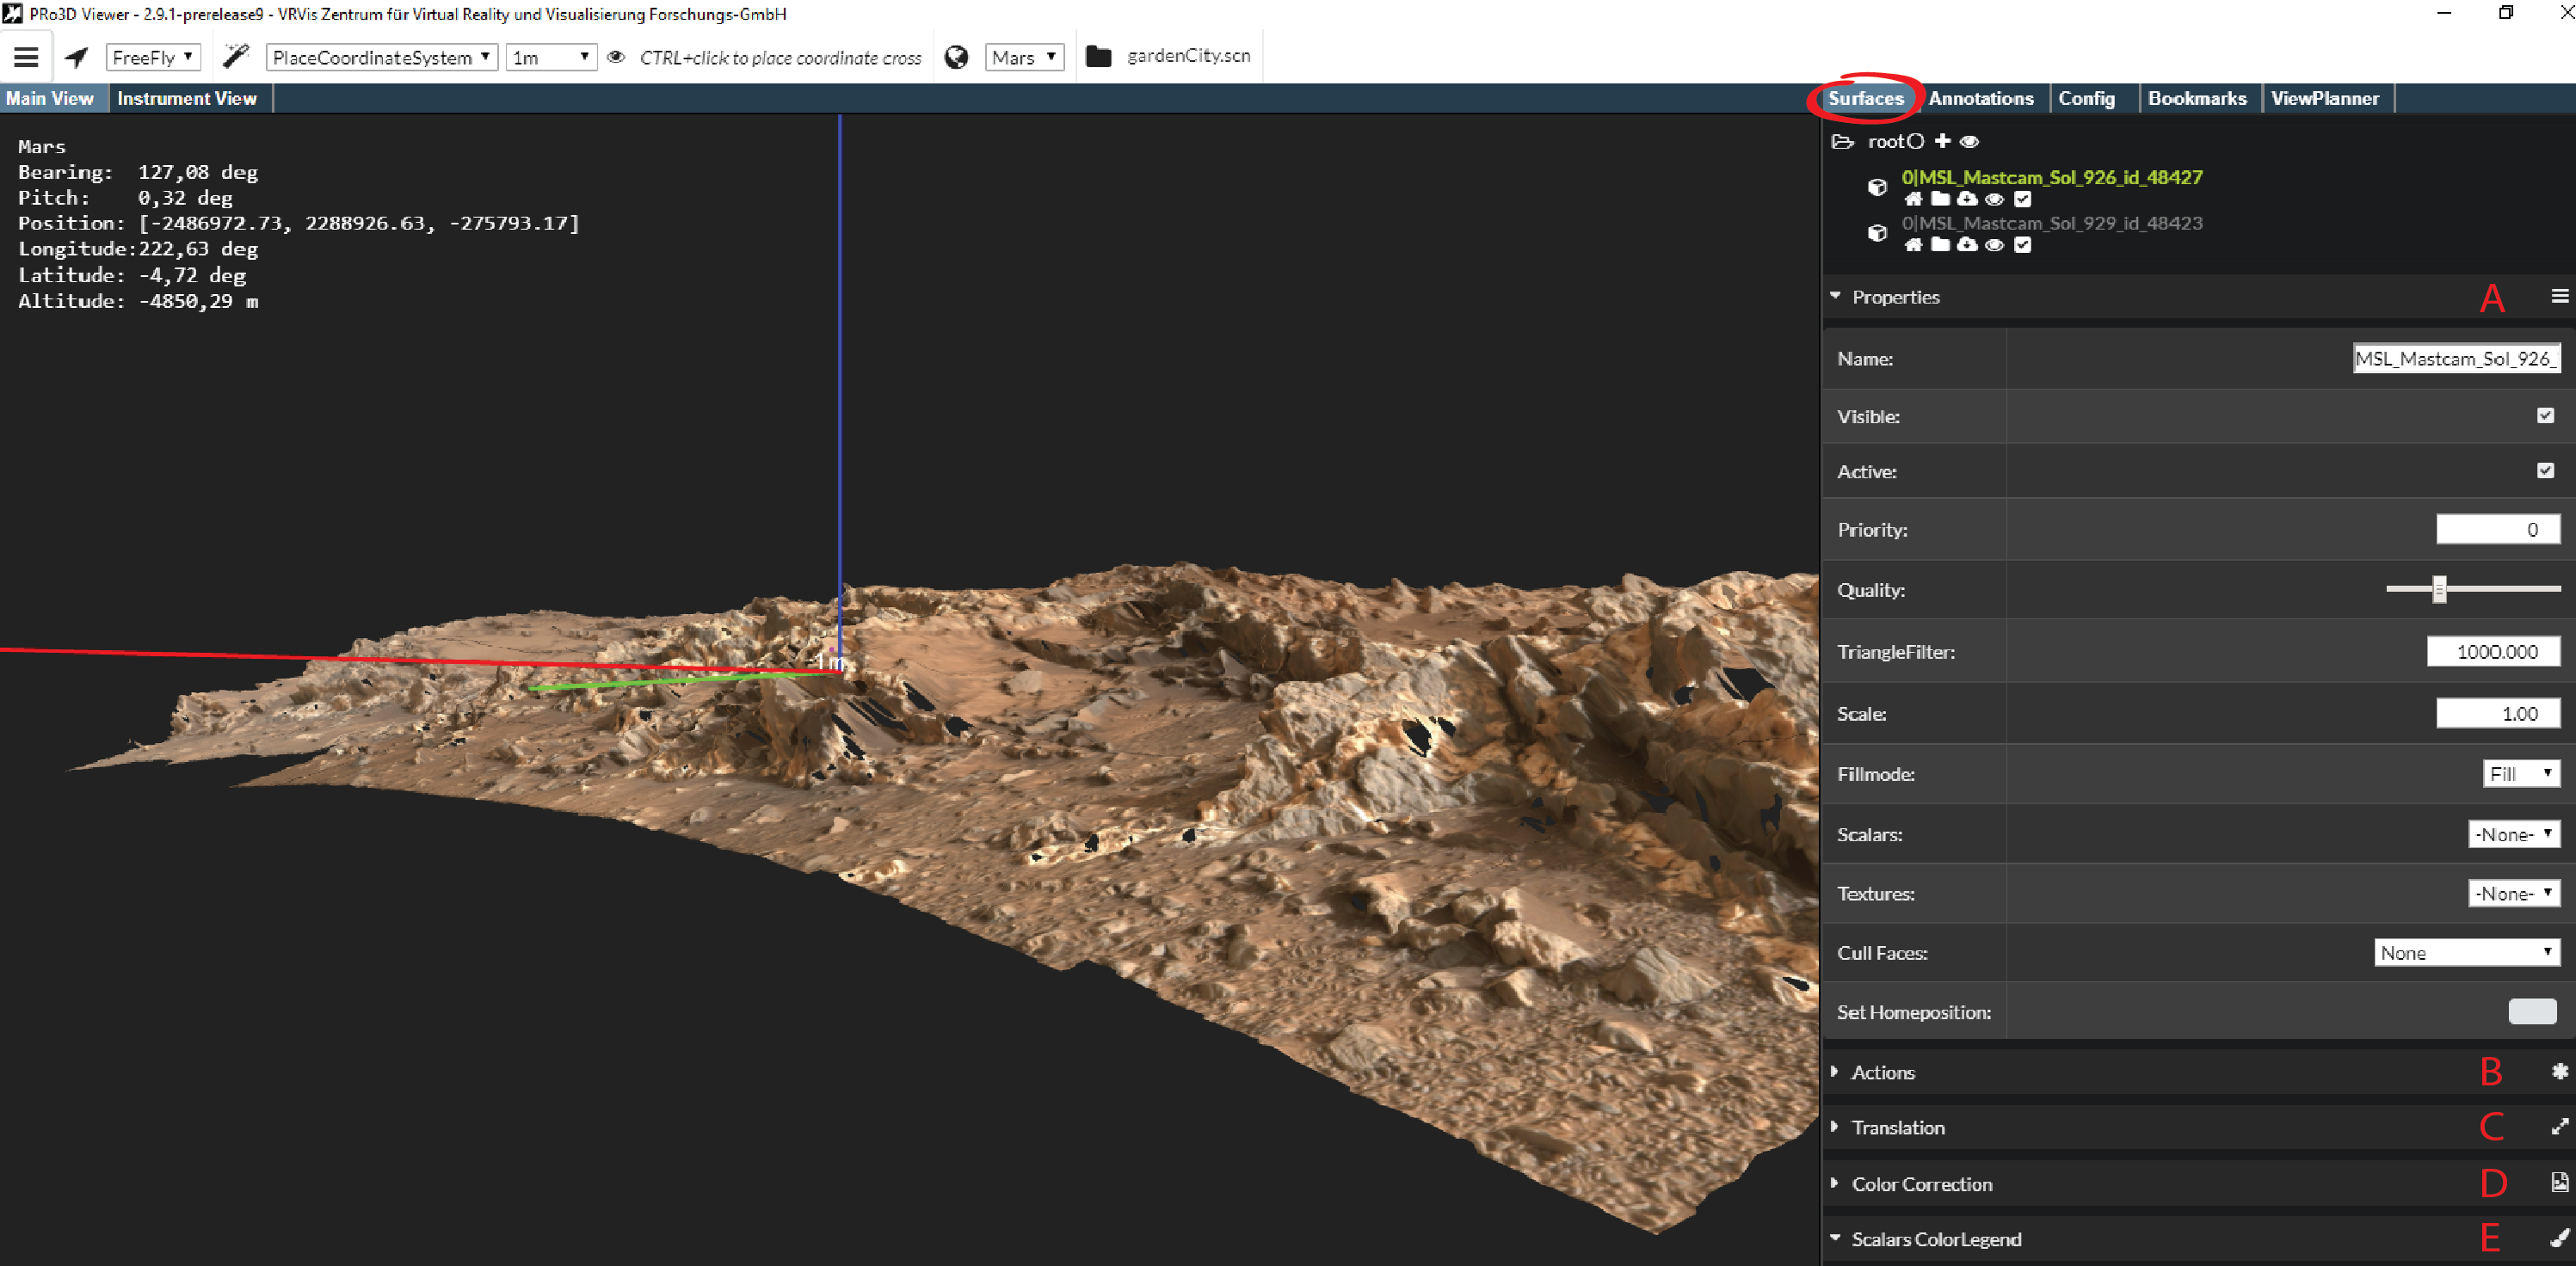
\includegraphics[width=0.5\textwidth]{pics/SurfacesAI.png}
    	\caption[Viewer Features Surfaces]{The surfaces tab.}
    	\label{fig:surfaces}
   \end{figure}

The listing shows all surfaces in the scene. You can classify them in any group and subgroup layers, described in Section~\ref{sec:grouping}.
You can select a surface by clicking on the surface's name. Then you can see the surface's properties in the properties panel and use the actions in the actions panel. 
It is also possible to select multiple surfaces by clicking the square icon in front of each surface. The selected surfaces have a green square in the list. The multiselection is used to move one ore more surfaces from one group to the active group.
Under the surface's name is a little menu:
\begin{itemize}
	\item \textit{FlyTo}: A click on the button triggers a FlyTo animation.
	\item \textit{portable}: This creates a folder hierarchy as used in the old viewer version. A scene file is created and the surfaces are copied to the surface folder.
	\item \textit{openFolder}: Opens the folder where the scene file resides.	
\end{itemize}

In the surface properties panel are some adjustments possible:
\begin{itemize}
	\item \textit{Name}: The surface's name. You can change it in the text field and press ``enter''.
	\item \textit{Visible}: The surface is visible (checked) or not (unchecked).
	\item \textit{Priority}:  Often multiple surfaces are available for a certain area on the planet surface. These surfaces represent the same piece of ground and typically overlap. This parameter allows to assign a priority to a surface to tell the graphics card which surface should be rendered in front. Lower numbers mean a higher priority in rendering, with 0 being the highest priority. You can also give the highest priority surface a ranking of, for instance, 0.1 (= 10cm) to make annotations more visible. The priority can be dynamically changed via the surface properties so you can try out what works best.
	\item \textit{Quality}: 
	\item \textit{TriangleSize}:
	\item \textit{FillMode}: You can switch between solid/ wireframe/ point rendering of the geometry.
	\item \textit{Scalars}:
	\item \textit{Textures}:
	\item \textit{Cull Faces}:
\end{itemize}

The surfaces actions are described in Section~\ref{sec:leafActions}.
%----------------------------------------------------------------------------------------
%	SubSection: Annotations
%----------------------------------------------------------------------------------------
\subsection{Annotations}
\label{sec:annotations}

\begin{figure}[h]
    	\centering
    		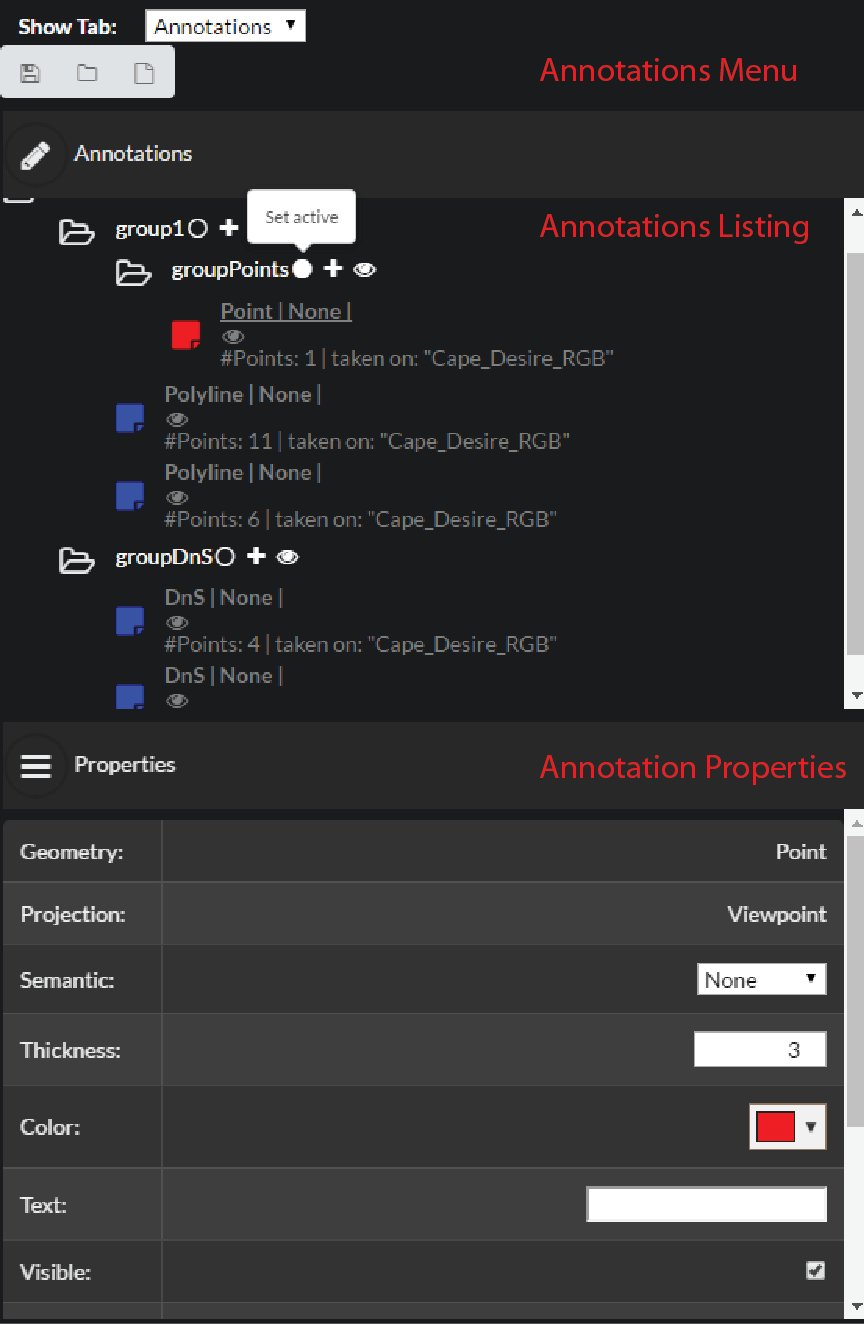
\includegraphics[width=0.5\textwidth]{pics/AnnotationsTabAI.png}
    	\caption[Viewer Features Annotations]{The annotations tab.}
    	\label{fig:annoProps}
   \end{figure}
	
The annotations tab consists of four parts (Figure~\ref{fig:annoProps}):

%----------------------------------------------------------------------------------------Annotations menu
\subsubsection{Annotations Menu}

In contrast to all other viewer features, the annotations are NOT saved in the scene file!
There is a separate menu on top of the annotations tab:
\begin{itemize}
	\item \textit{Save Annotations}: Opens a ``Save As'' window. Give your annotations xml file a name and click the ``Save'' button.
	\item \textit{Load Annotations}: Select the annotations xml file and press the ``Open'' button. 
	\item \textit{Clear Annotation List}: This clears the whole annotation list.
\end{itemize}

%----------------------------------------------------------------------------------------Annotations listing
\subsubsection{Annotations Listing}

The listing shows all annotations in the scene. You can classify them in any group and subgroup layers, described in Section~\ref{sec:grouping}.
You can select an annotation by clicking on the annotation's name. Then you can see the annotation's properties in the properties panel and use the actions in the actions panel. 
It is also possible to select more annotations by clicking the square icon in front of each annotation. The selected annotations have a green color in the viewer and a green square in the list. The multiselection is used to move one ore more annotations from one group to the active group.

%----------------------------------------------------------------------------------------Annotations properties
\subsubsection{Annotations Properties}

The properties of the selected annotation (click on annotation's name) are shown. There you can get information and change some of the settings:
\begin{itemize}
	\item \textit{Geometry}: Shows the annotation mode (described in Section~\ref{sec:drawAnnotation}). This is not changeable retrospectively.
	\item \textit{Projection}: Shows the projection which determines the direction of the picking ray (described in Section~\ref{sec:drawAnnotation}, shown in Figure~\ref{fig:projection}). This is not changeable retrospectively.
	\item \textit{Semantic}: 
	\item \textit{Thickness}: You can change the annotation's line thickness.
	\item \textit{Color}: You can change the annotation's color.
	\item \textit{Text}: You can append a note. Write in the text field and press ``Enter''. The note will appear next to the annotation in the viewer. 
	\item \textit{Visible}: The annotation is visible (checked) or not (unchecked).
	\item \textit{ShowDnS}: For each annotation with more than three picking points Dip and Strike information (Section~\ref{sec:drawAnnotation}) is available. The DnS is visible (checked) or not (unchecked).
	\item \textit{Height}:  The height between the annotation's start and end point.
	\item \textit{HeightDelta}: The height difference between the highest and lowest point of the projected line.
	\item \textit{Length}: The sum of direct distances between the picking points.
	\item \textit{WayLength}: The sum of projected distances between the picking points.
\end{itemize}

The annotations actions are described in Section~\ref{sec:leafActions}.

%----------------------------------------------------------------------------------------Import AnnotationGroups
\subsubsection{Import Annotations from old viewer versions} 

To import annotations from old scene files click the ``browse'' button in the \textbf{ImportAnnotationGroups} section in the Scene Menu (Figure~\ref{fig:StartMenu}). This opens a folder browser dialog, where you can select an old scene file an click ''Open''.
The annotations are loaded in the same group hierarchy to the ``root'' group.


%----------------------------------------------------------------------------------------
%	SubSection: ViewPlanner
%----------------------------------------------------------------------------------------
%\subsection{ViewPlanner}
%\label{sec:viewPlanner}

%----------------------------------------------------------------------------------------
%	SubSection: Bookmarks
%----------------------------------------------------------------------------------------
\subsection{Bookmarks}
\label{sec:bookmarks}

\begin{figure}[h]
    	\centering
    		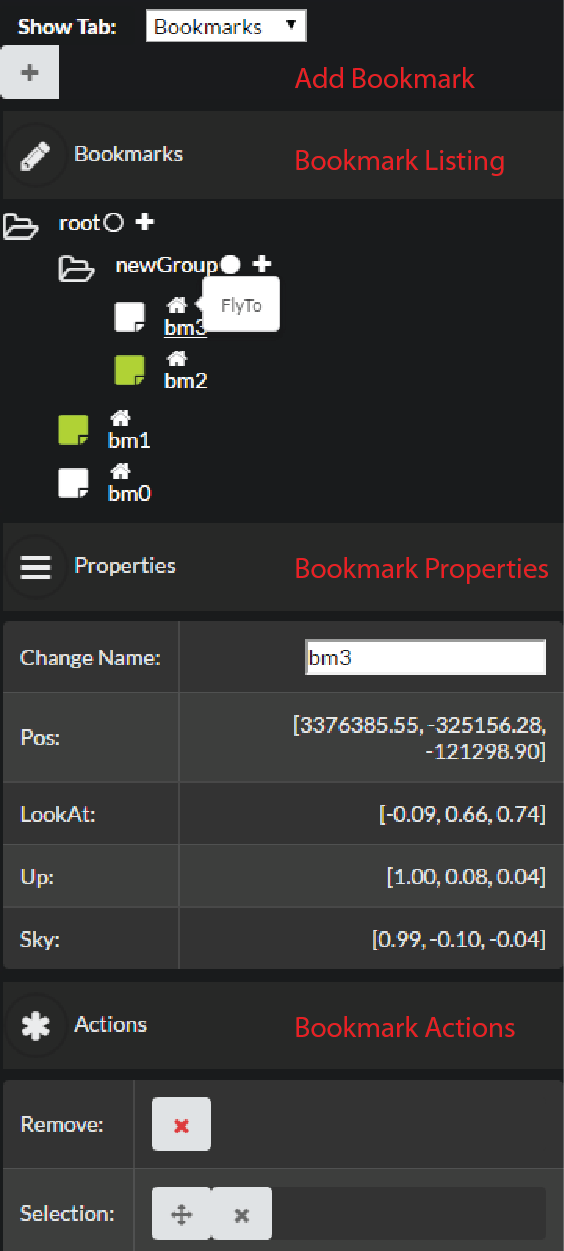
\includegraphics[width=0.5\textwidth]{pics/bookmarks.png}
    	\caption[Viewer Features Bookmarks]{The bookmarks tab.}
    	\label{fig:bookmarks}
   \end{figure}
	
Bookmarks enable the user to record a certain camera viewpoint.
To add a new bookmark click the ``+'' button on top of the tab (Figure~\ref{fig:bookmarks}). The new bookmark is added to the active group in the bookmarks listing.
To view the bookmark's properties and actions click on the bookmark's name. Clicking the ``house'' button beside the bookmark's name triggers a FlyTo. For multiselection click on the bookmark's square icons.

%----------------------------------------------------------------------------------------
%	SubSection: Viewer Configuration
%----------------------------------------------------------------------------------------
\subsection{Viewer Configuration}
\label{sec:config}

\begin{figure}[h]
    	\centering
    		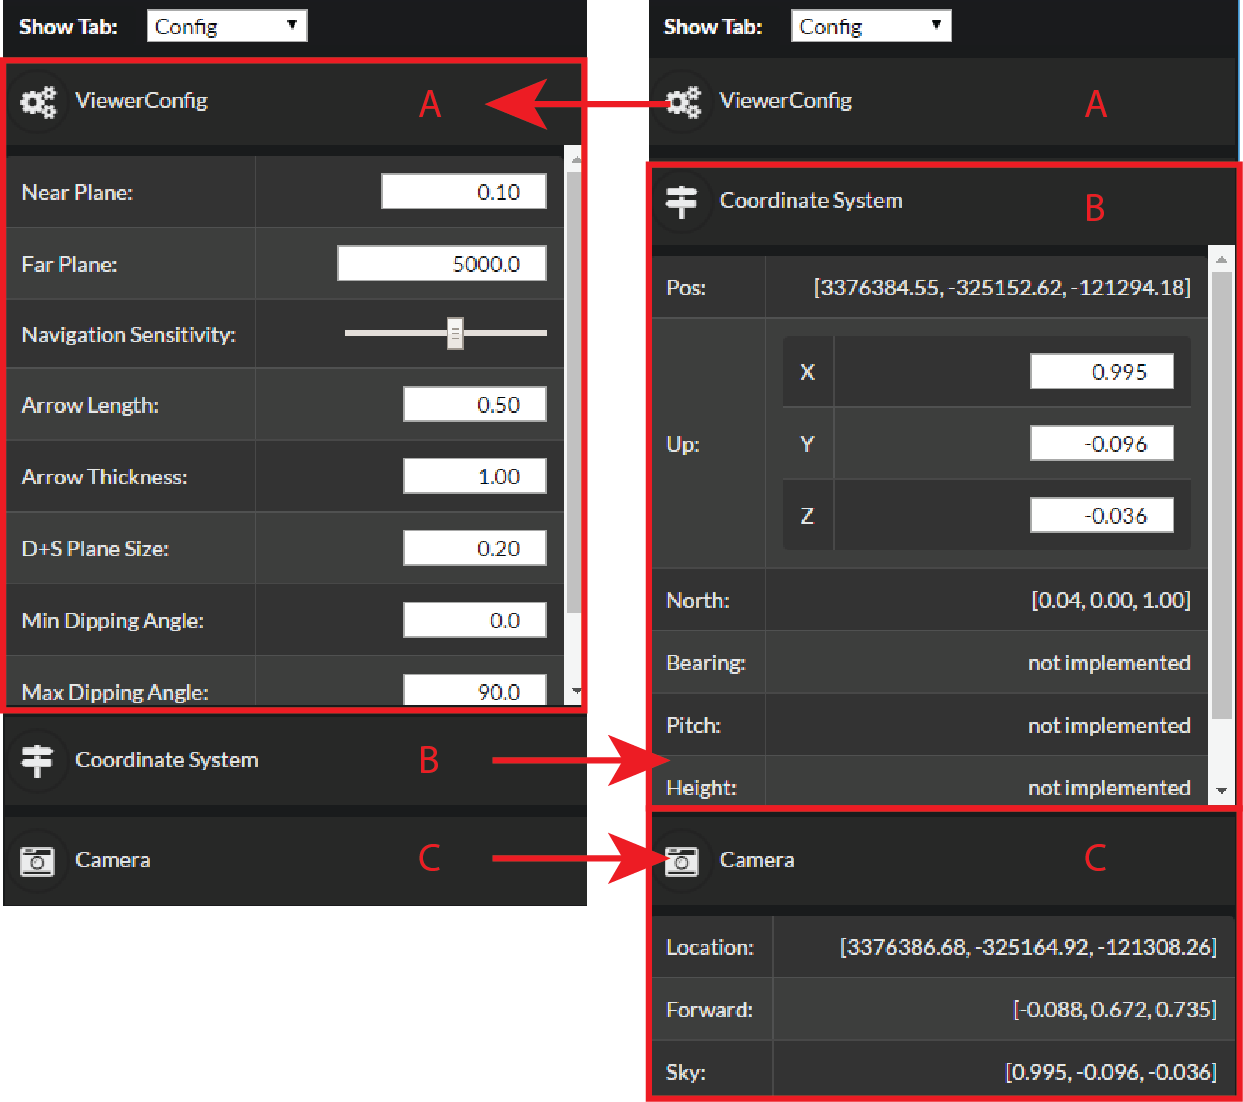
\includegraphics[width=0.8\textwidth]{pics/ViewerConfigAI.png}
    	\caption[Viewer Configuration]{The ``Config'' Menu with the ViewerConfiguration (A), Coordinate System (B) and Camera settings (C).}
    	\label{fig:viewerConfig}
   \end{figure}

To edit the viewer properties, select ``Config'' in the viewer features drop down menu (Figure~\ref{fig:featureMenu}).
There are three submenus in the config tab:
\begin{itemize}
	\item ViewerConfig (A in Figure~\ref{fig:viewerConfig})
	\item Coordinate System (B in Figure~\ref{fig:viewerConfig})
	\item Camera (C in Figure~\ref{fig:viewerConfig})
\end{itemize}

%----------------------------------------------------------------------------------------Viewer Config
\subsubsection{ViewerConfig} 

A set of major viewer properties can be adjusted:
\begin{itemize}
	\item \textit{Near/Far Plane}: The near- and the far clipping plane are automatically adjusted according to the data to be rendered. The set values are shown in the config panel and can be adjusted afterwards. 
	\item \textit{Navigation Sensitivity}: The navigation sensitivity can also be adjusted by PageUp and PageDown keys. 
	\item \textit{Arrow Length/Thickness}: The arrow length and thickness is set for up- and north vectors, dip and strike vectors and the up- and lookAt vectors in the rover view planner. 
	\item \textit{D+S Plane Size}: The dip and strike measurements plane size, described in Section~\ref{sec:drawAnnotation}
 (Figure~\ref{fig:drawAnnotations}).
	\item \textit{Min/Max Dipping Angle}: The dip and strike measurements dipping angle range. The dipping angle is coded into the color of the disc and arrow of a measurement (Figure~\ref{fig:drawAnnotations}).
	\item \textit{Lod Colors}: The different levels of detail of the surface geometry can be colored in different shades of red.
			This helps to evaluate the export of OPC data.
\end{itemize}

%----------------------------------------------------------------------------------------Coordinate System
\subsubsection{Coordinate System} 

The coordinate system menu shows the position, Up- and North Vector of the coordinate system described in Section~\ref{sec:placeCS}, shown in Figure~\ref{fig:coordinateSystem}.
The Up- and the North Vector are used for the projection measurements (Figure~\ref{fig:drawAnnotations}). Initially the Up Vector's direction is set in the positive z-direction and the North Vector's in the positive y-direction. But you can manipulate the Up Vector manually for different data. Both vectors are computed automatically with picking of a new position for the coordinate system. The north vector is further relevant for bearing measurements. % and the rover placement in the View Planner (see Section 4.6). 

%----------------------------------------------------------------------------------------Camera
\subsubsection{Camera} 

The Camera submenu shows the Location, Forward- and Sky vector of the main camera.
%----------------------------------------------------------------------------------------
%	SubSection: Grouping
%----------------------------------------------------------------------------------------
\subsection{Grouping}
\label{sec:grouping}

\begin{figure}[h]
    	\centering
    		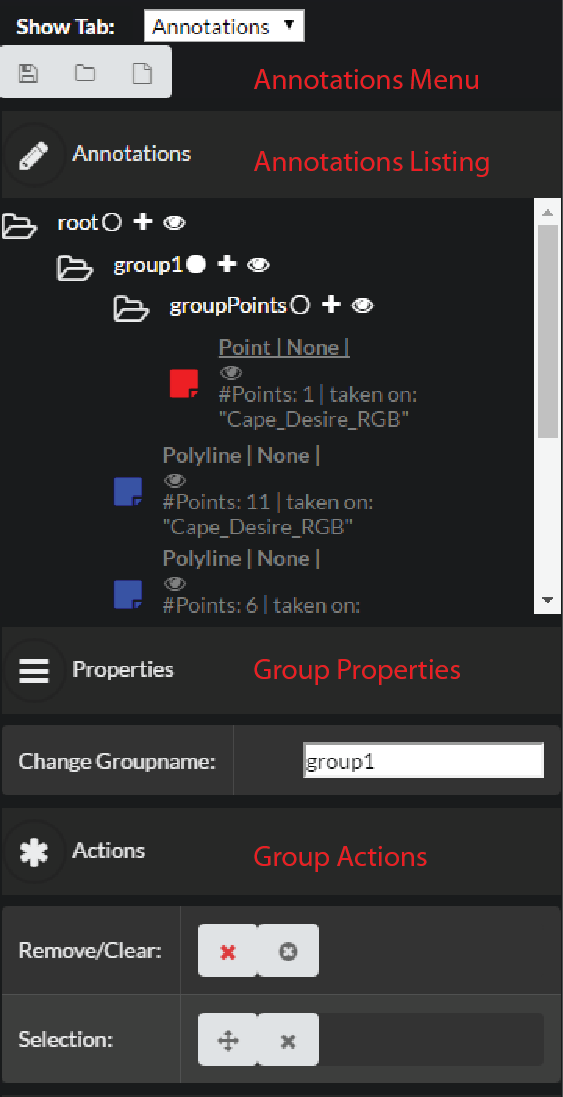
\includegraphics[width=0.5\textwidth]{pics/GroupsProperties.png}
    	\caption[Viewer Features]{The group properties and actions.}
    	\label{fig:groupProps}
   \end{figure}

Grouping is possible for surfaces, annotations and bookmarks.
The ``root'' group is the highest level where you can add leafs and subgroups (Figure~\ref{fig:groupProps}).
Each group has a context menu:
\begin{itemize}
	\item \textit{Set Active}: The active group gets the new leaf. Per default the ``root'' is active.
	\item \textit{Add Group}: Adds a new and empty subgroup.
	\item \textit{Toggle Group}: Sets all leafs in this group and its subgroups invisible.
\end{itemize}

%----------------------------------------------------------------------------------------Group actions
\subsubsection{Group Actions}
\label{sec:groupActions}

\begin{itemize}
	\item \textit{Remove}: Removes the group with all its leafs and subgroups.
	\item \textit{Clear}: Removes all leafs and subgroups from group but retains the empty group. 
	\item \textit{Selection: Move}: Moves all selected leafs (green squares) to the active group.
	\item \textit{Selection: Clear}: Clears the selection (the leafs were not removed).
\end{itemize}
	
%----------------------------------------------------------------------------------------Leaf actions
\subsubsection{Leaf Actions}
\label{sec:leafActions}

\begin{itemize}
	\item \textit{Remove}: Removes the leaf.
	\item \textit{Selection: Move}: Moves all selected leafs (green squares) to the active group.
	\item \textit{Selection: Clear}: Clears the selection (the leafs were not removed).
\end{itemize}

%----------------------------------------------------------------------------------------
%	Section: Minerva
%----------------------------------------------------------------------------------------
%----------------------------------------------------------------------------------------
%	Section: Minerva
%----------------------------------------------------------------------------------------
\section{Minerva}

\begin{figure}[h]
    	\centering
    		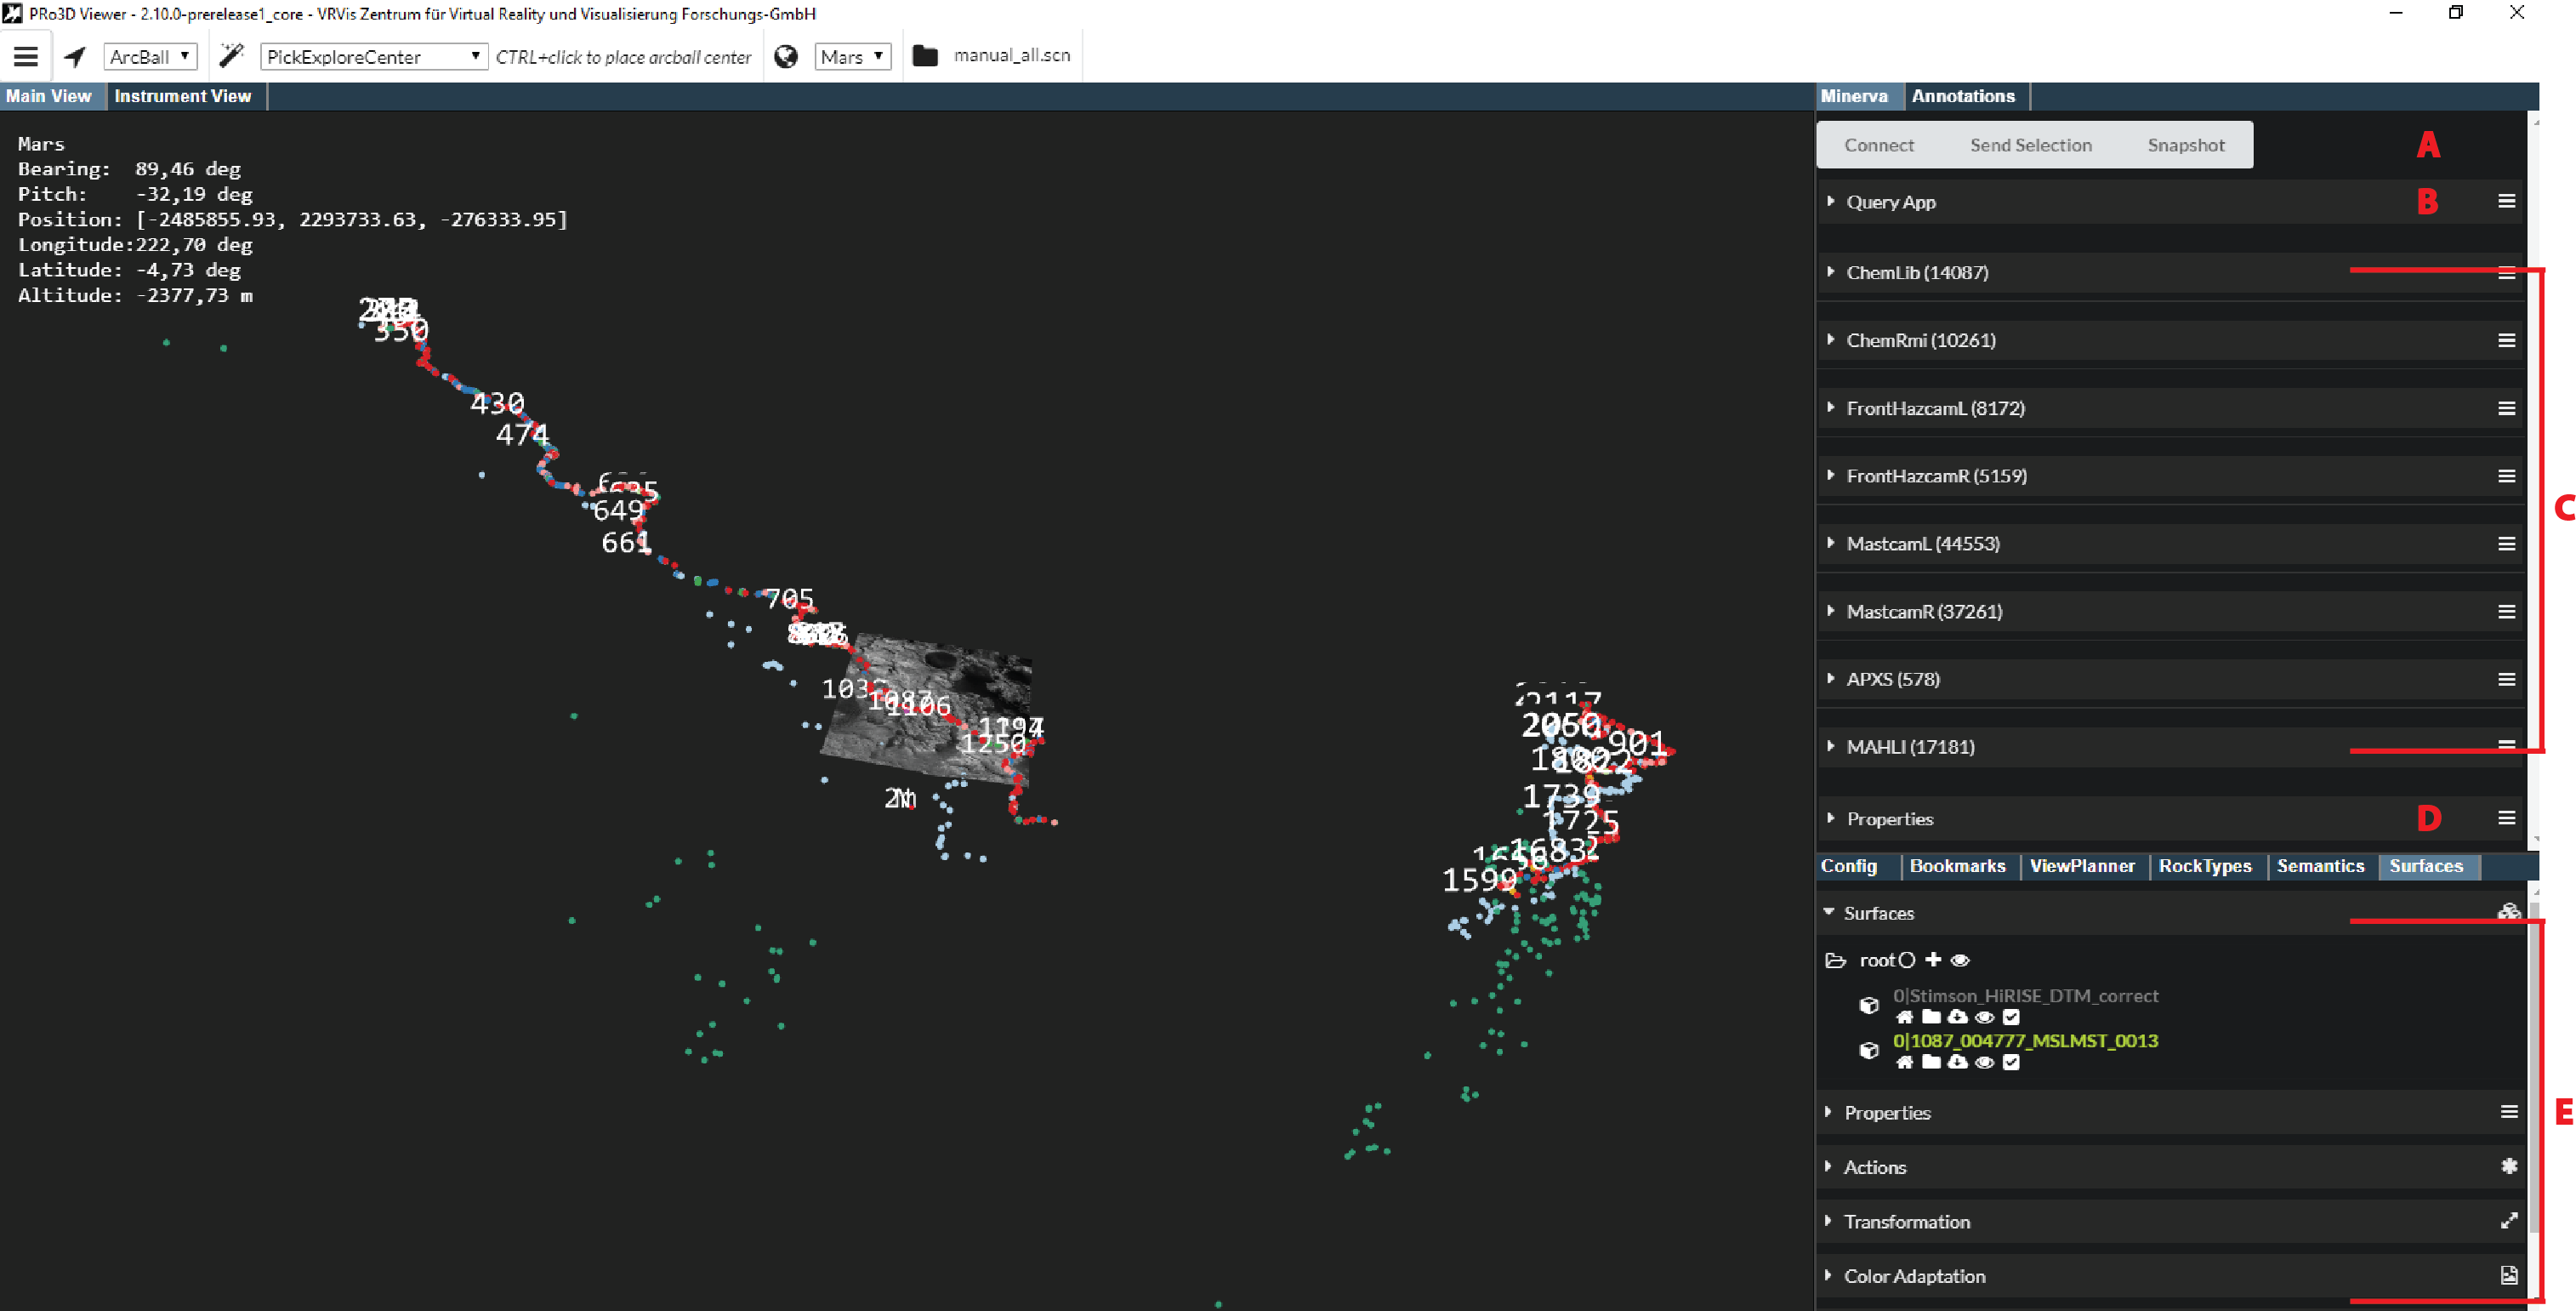
\includegraphics[width=1\textwidth]{pics/MinervaAI.png}
    	\caption[Start Minerva]{The Minerva Application. The Main View (left) shows the surface data with the products. There are different interaction possibilities for the products in the Minerva tab (right). A: Visplore communication, B: Query App to reduce the shown products by the mean of different criteria, C: Product listing, D: Properties of the last selected product, E: Surface tab.  }
    	\label{fig:StartMinerva}
   \end{figure}

%----------------------------------------------------------------------------------------
%	SubSection: Start Minerva
%----------------------------------------------------------------------------------------
\subsection{Start Minerva}
\label{sec:startMinerva}

Before you start the Minerva Application make sure that the \textbf{dump.csv} file is in the \textbf{\path{Release\netcoreapp2.0\MinervaData}} folder.
Then start the viewer by clicking the PRo3D.exe as described in Section~\ref{sec:startViewer}. The Minerva data from the dump.csv file is loaded and the products are listed in the ``Minerva'' tab as shown in Figure~\ref{fig:StartMinerva} C.  Load the surface data as described in Section~\ref{sec:addSurface}.
How to explore and adjust the surfaces is described in Section~\ref{sec:surfaces}.
You can save the scene as described in Section~\ref{sec:addSurface}.

%----------------------------------------------------------------------------------------
%	SubSection: Minerva Features
%----------------------------------------------------------------------------------------
\subsection{Minerva Features}
\label{sec:minervaFatures}

%----------------------------------------------------------------------------------------Visplore
\subsubsection{Visplore}

Visplore is a powerful visual analytics tool that allows the handling of huge and heterogeneous data and provides different perspectives onto the data that help finding causalities and allow an easy examination of the data's plausibility. 
For this project an interface was implemented that allows an interconnected workflow between PRo3D and Visplore.
To communicate with Visplore use the tree buttons shown in Figure~\ref{fig:StartMinerva} A:
\begin{itemize}
	\item \textbf{Connect:} Connect to Visplore.
	\item \textbf{Send Selection:} Send the selected products to Visplore.
	\item \textbf{Snapshot:} Send a snapshot of the MainView to the Visplore MapView.
\end{itemize}
For more information how to use Visplore for Minerva, please refer to the Visplore manual.

%----------------------------------------------------------------------------------------Query App
\subsubsection{QueryApp}
	
	\begin{figure}[h]
    	\centering
    		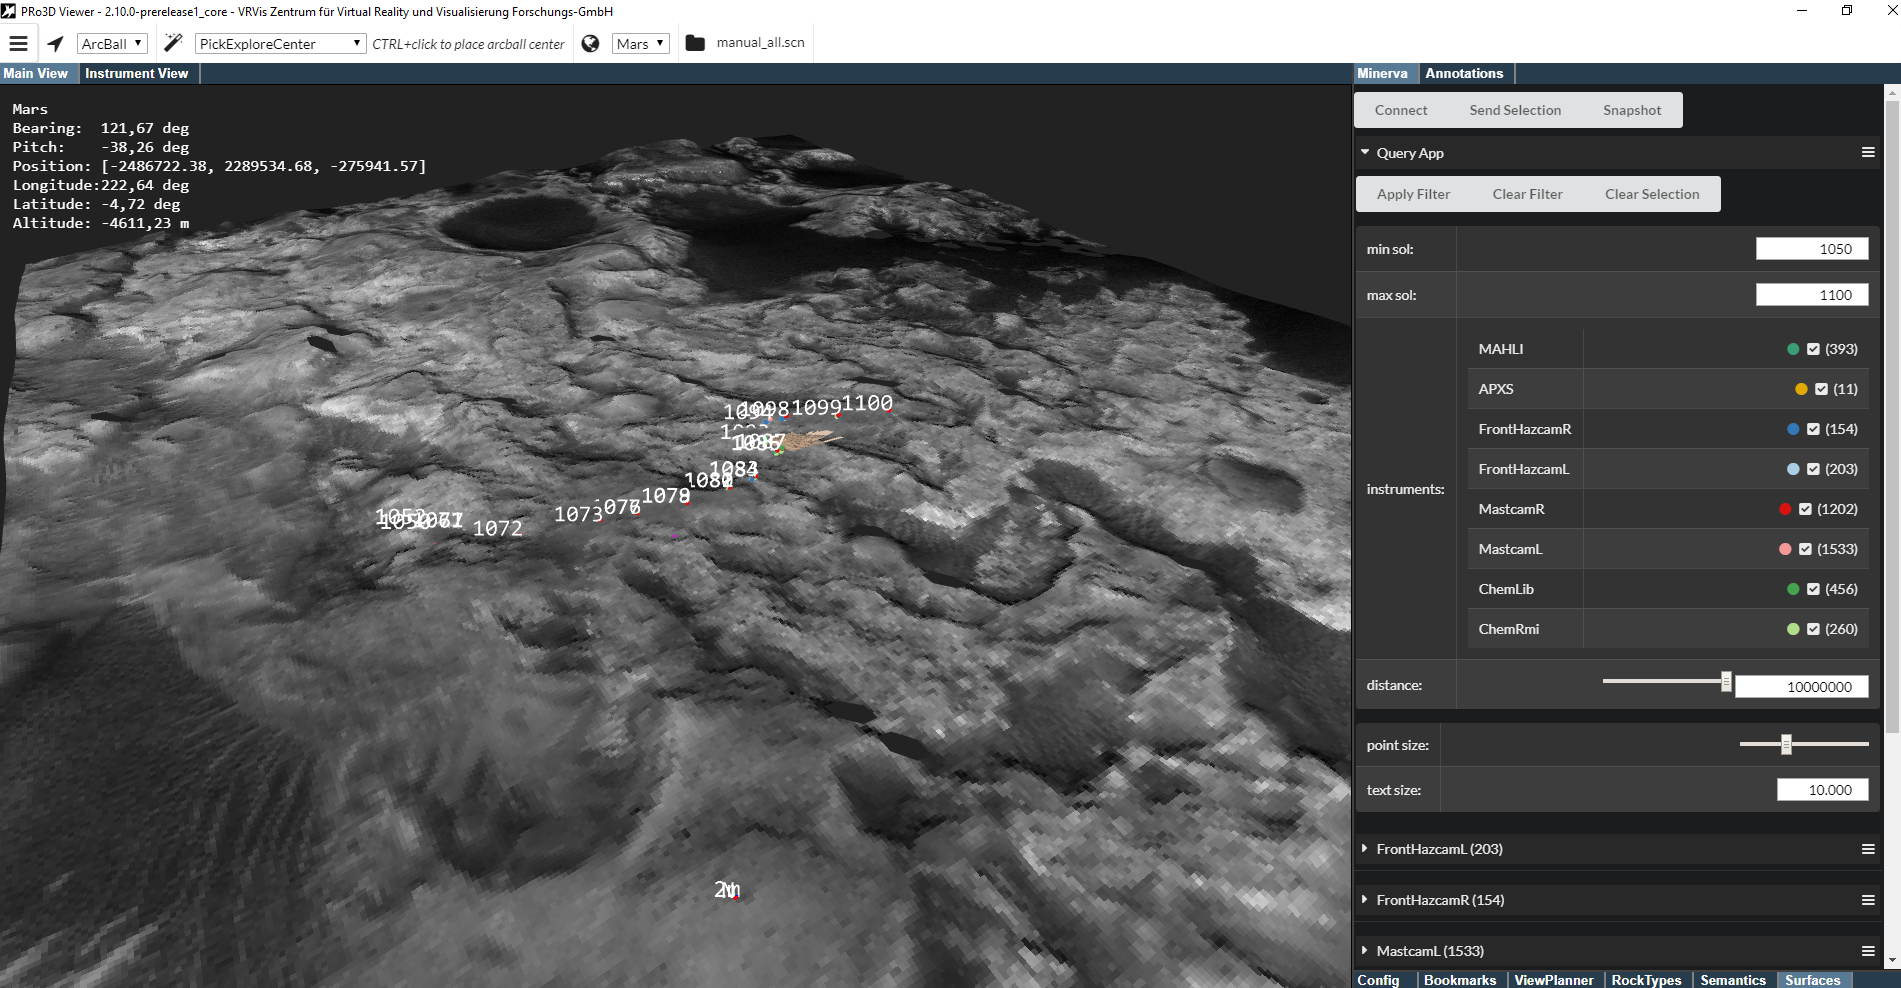
\includegraphics[width=1\textwidth]{pics/QueryApp.png}
    	\caption[Query App]{The Query App (right).}
    	\label{fig:QueryApp}
   \end{figure}

The Query App provides the possibility to cut down the number of shown products by the mean of different criteria. These criteria are:
\begin{itemize}
	\item \textbf{min- and max sol:} All products with sol numbers in the given range are shown.
	\item \textbf{instruments:} Only the products with checked instruments are shown.
	\item \textbf{distance:} The distance between the camera location and the shown products is less than the entered distance value.
\end{itemize}
You can use one ore more criteria and press the \textbf{``ApplyFilter''} button in top of the Query App menu. Now only the filtered products are shown. Change the queries and click ``ApplyFilter'' again to change the shown products. To get all products click the \textbf{``ClearFilter''} button. 
You can also change the \textbf{point size} of the rendered products in the Main View, and the \textbf{text size} of the shown sol numbers.

%----------------------------------------------------------------------------------------Product Listing
\subsubsection{Product Listing and Selection}
\label{sec:selection}

\begin{figure}[h]
				\centering
					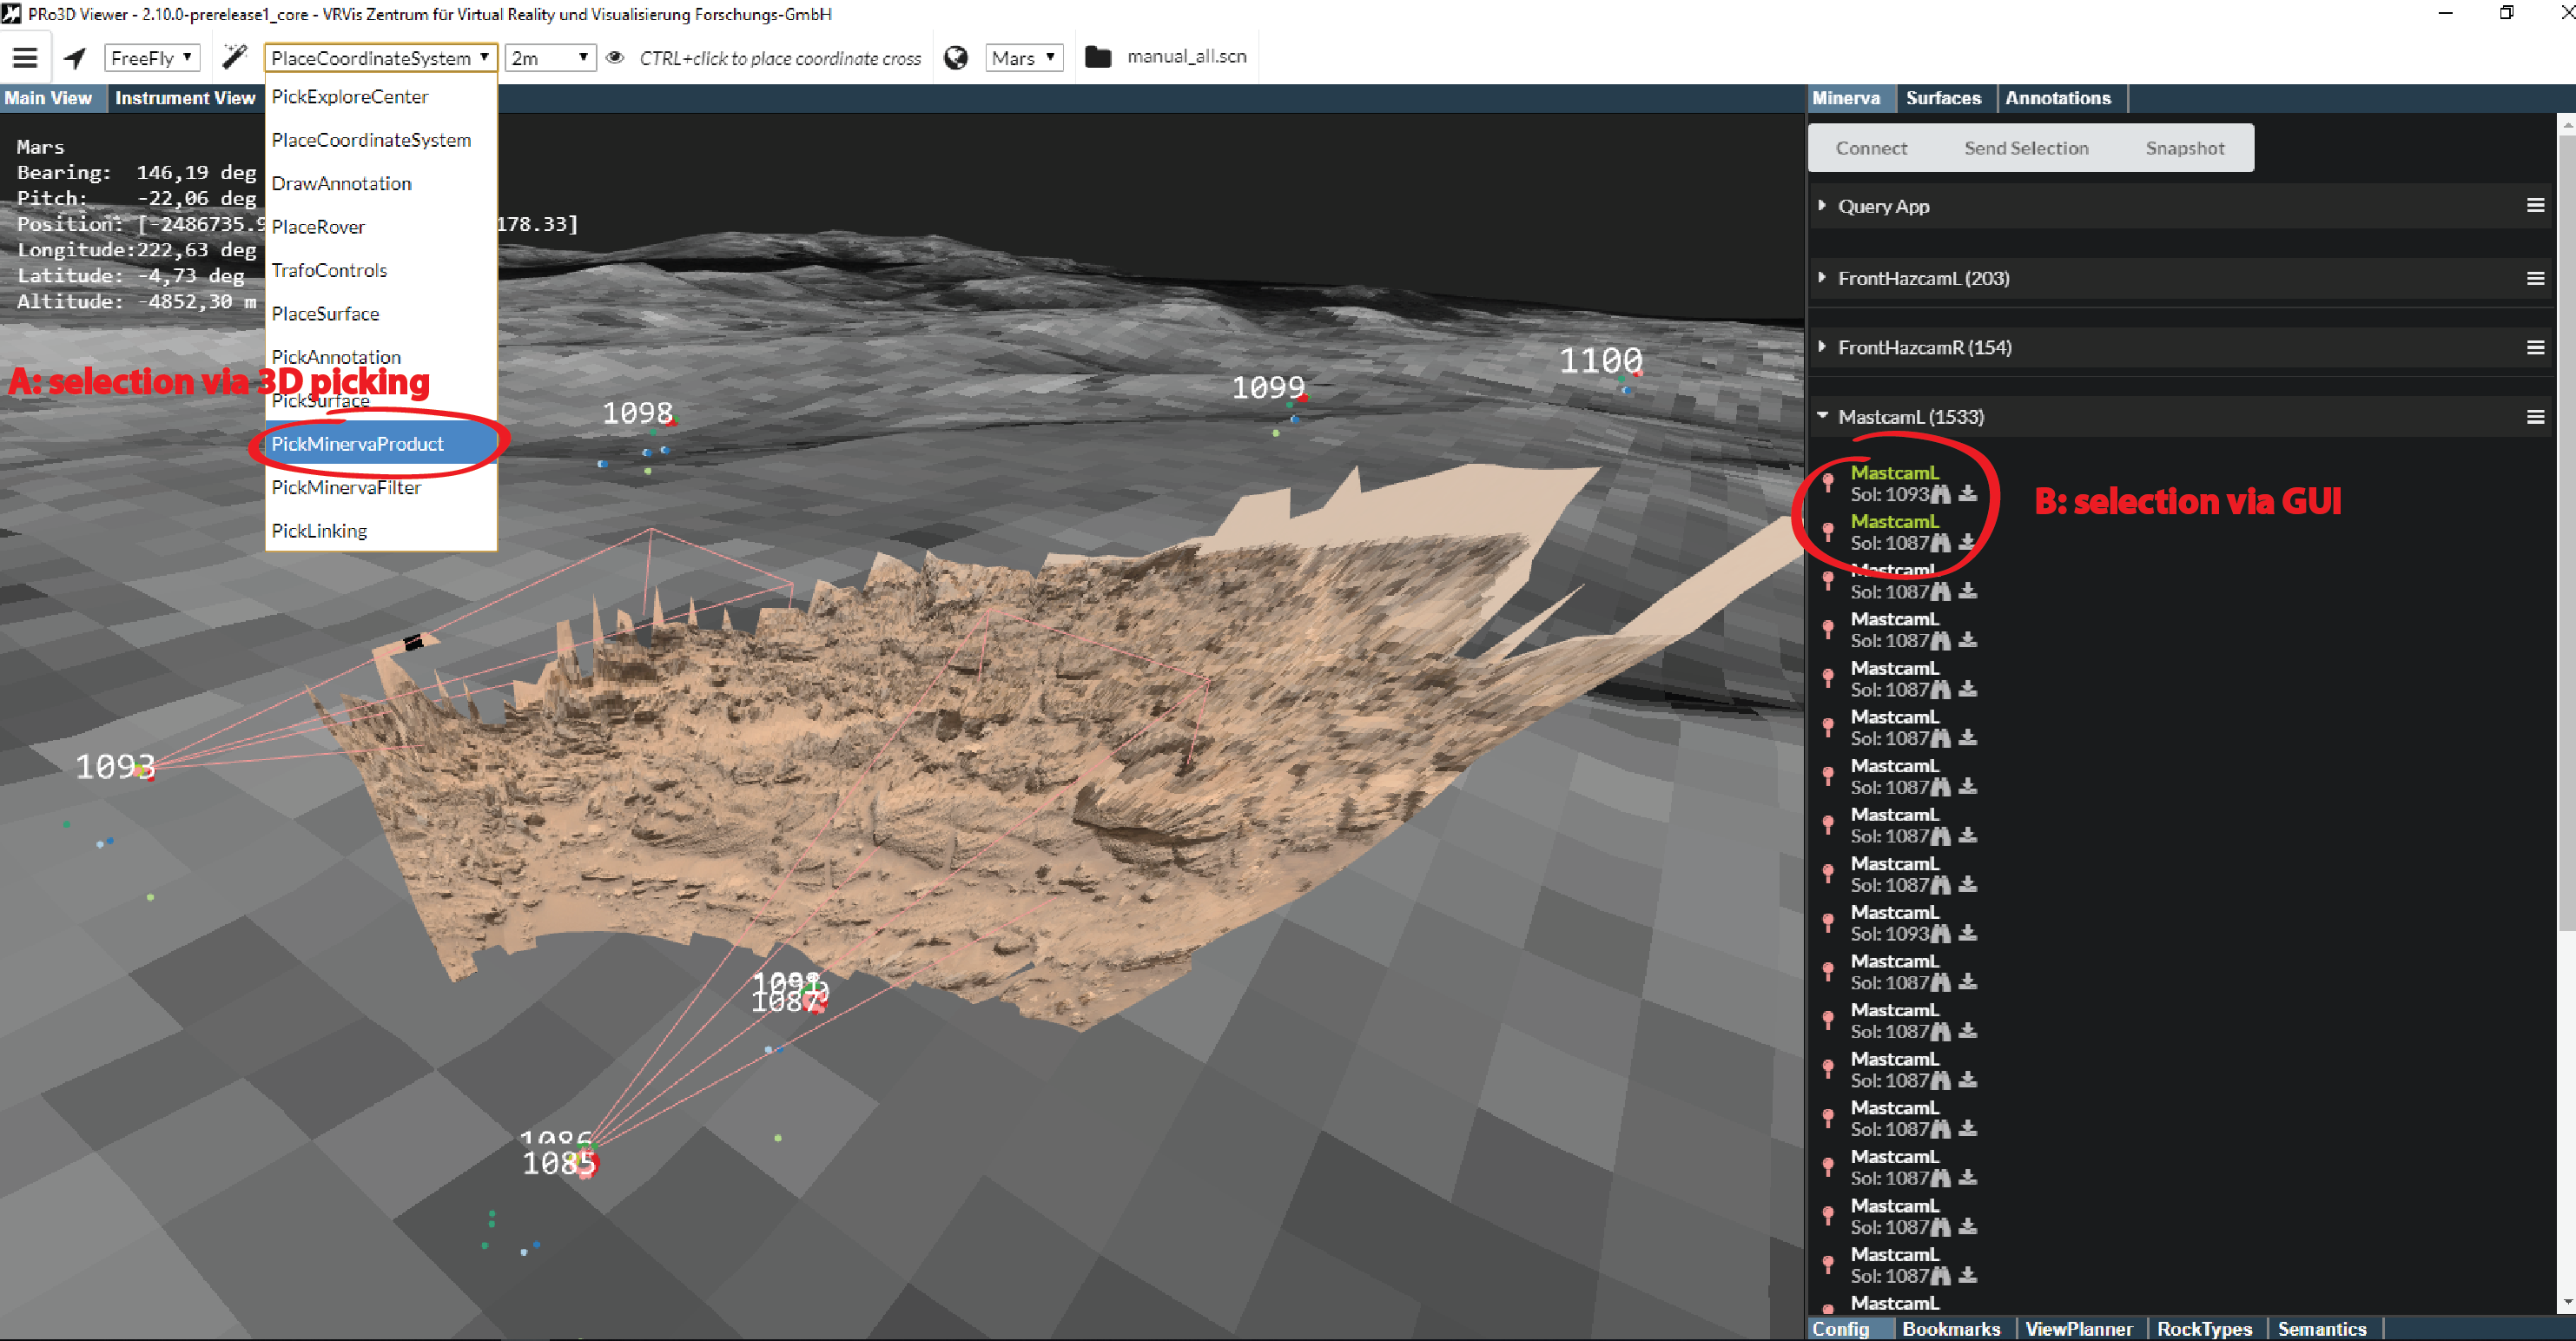
\includegraphics[width=1\textwidth]{pics/ListingAI.png}
				\caption[Product Listing]{The products are grouped by instruments. A product can either be selected in the listing (B) or in the Main View (A). }
				\label{fig:ProductListing}
		 \end{figure}
		
The products are grouped in the gui by their instruments (Figure~\ref{fig:StartMinerva} C) where the first 20 products for each instrument are listed.
You can select single products by clicking on the products's name, which turns its color to green. Or you can set ``PickMinervaProduct'' in the actions menu (Figure~\ref{fig:ProductListing}), press CTRL+LMB and pick the product in the main view. Then you can see the product's properties in the properties panel, described in the next Section~\ref{sec:productProps}. 

\begin{figure}[h]
				\centering
					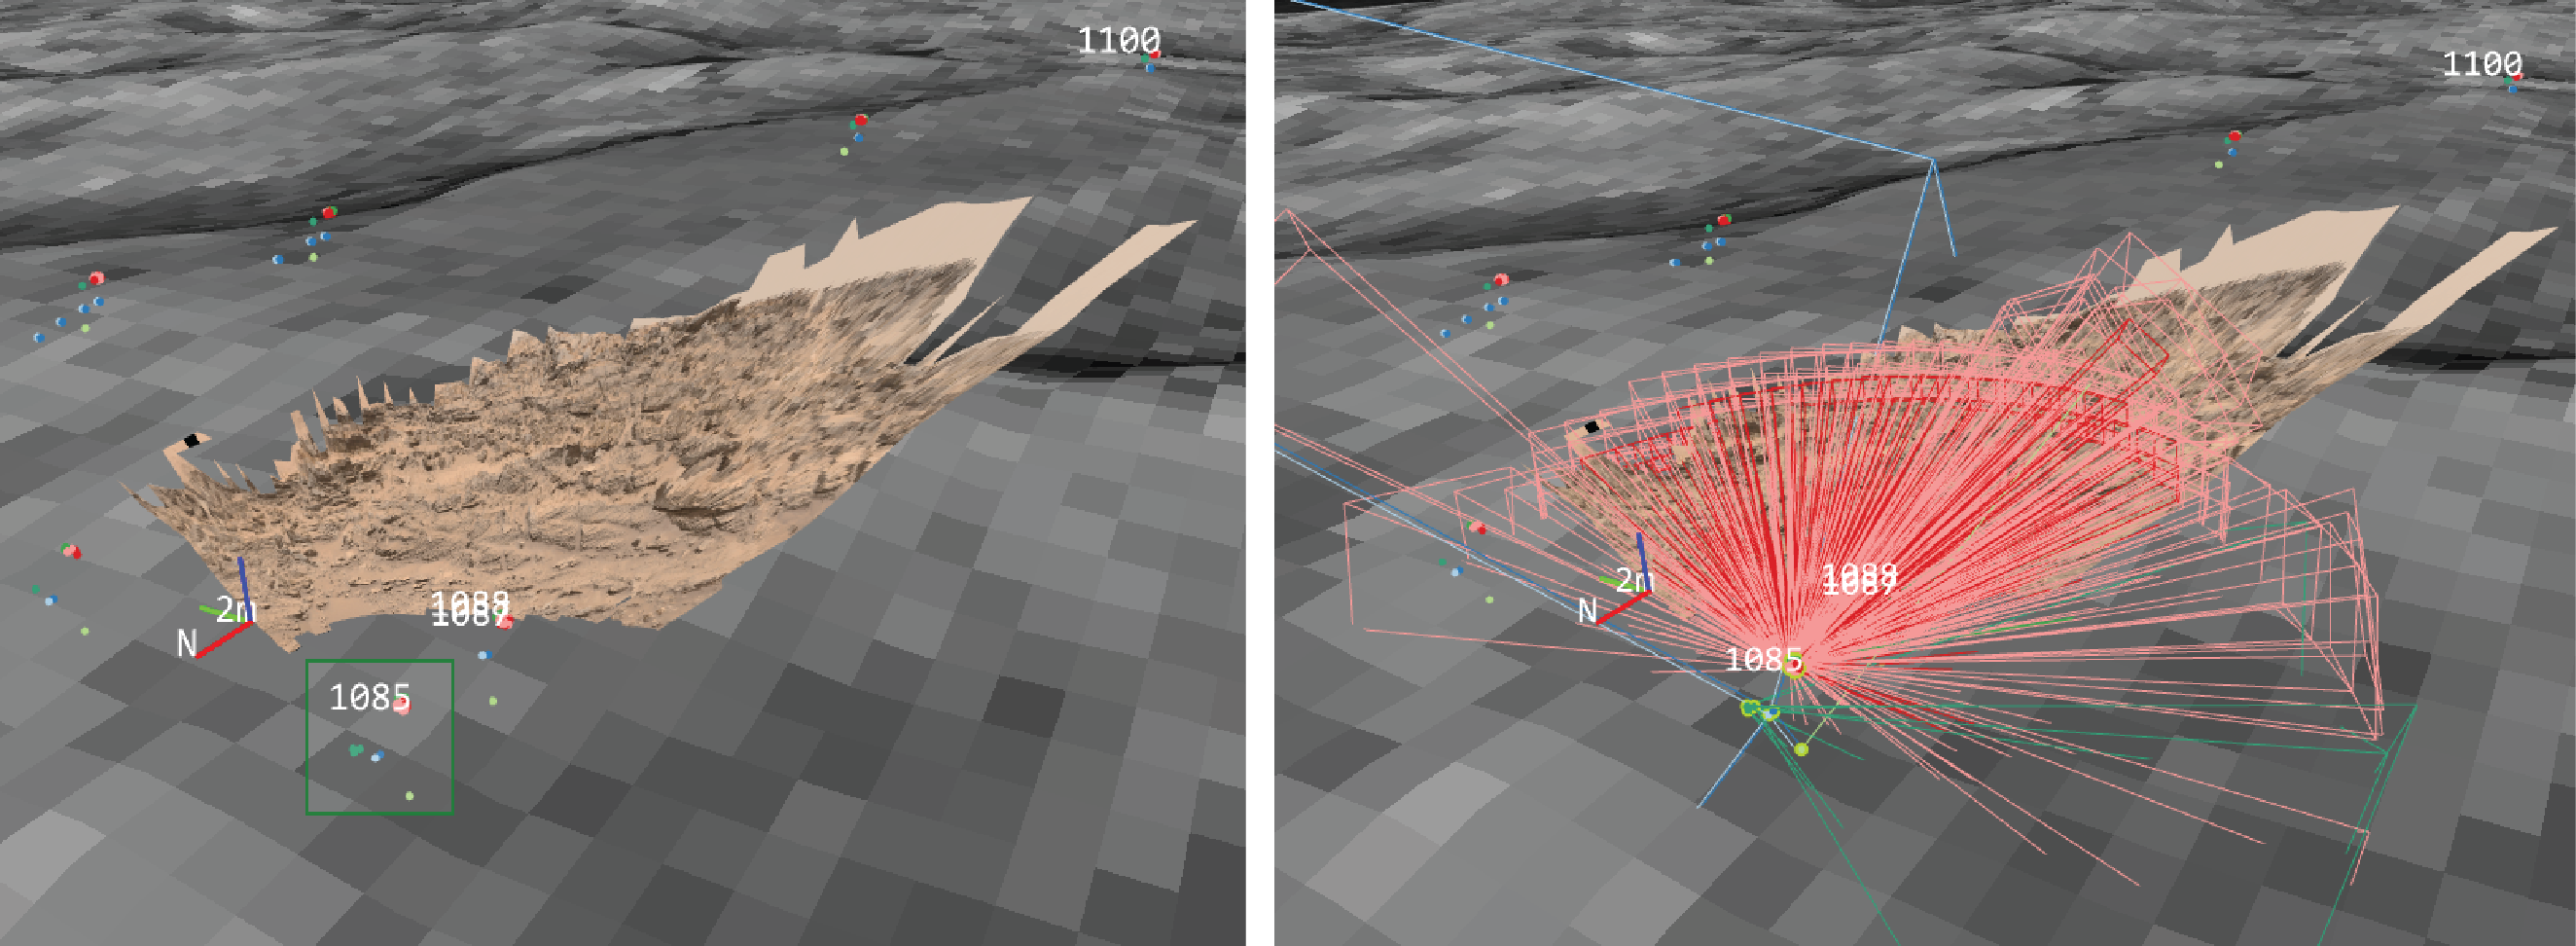
\includegraphics[width=1\textwidth]{pics/MultiSelAI.png}
				\caption[Multi Selection]{A rectangle is spanned over multiple products (left). All products selected by the rectangle (right).}
				\label{fig:MultiSel}
		 \end{figure}
		
It is also possible to select multiple products. Press SHIFT+LMB and drag a rectangle (Figure~\ref{fig:MultiSel} left). When you release the LMB, all products in this area are selected (Figure~\ref{fig:MultiSel} right). \\
Under the products's name is a little menu:
\begin{itemize}
  \item \textbf{The Sol Number}
	\item \textbf{FlyTo}: A click on the button triggers a FlyTo animation.
	\item \textbf{GetTif}: Downloads the product's tif image.
\end{itemize}

	
	
%----------------------------------------------------------------------------------------Product Properties
\subsubsection{Product Properties}
\label{sec:productProps}

\begin{figure}[h]
				\centering
					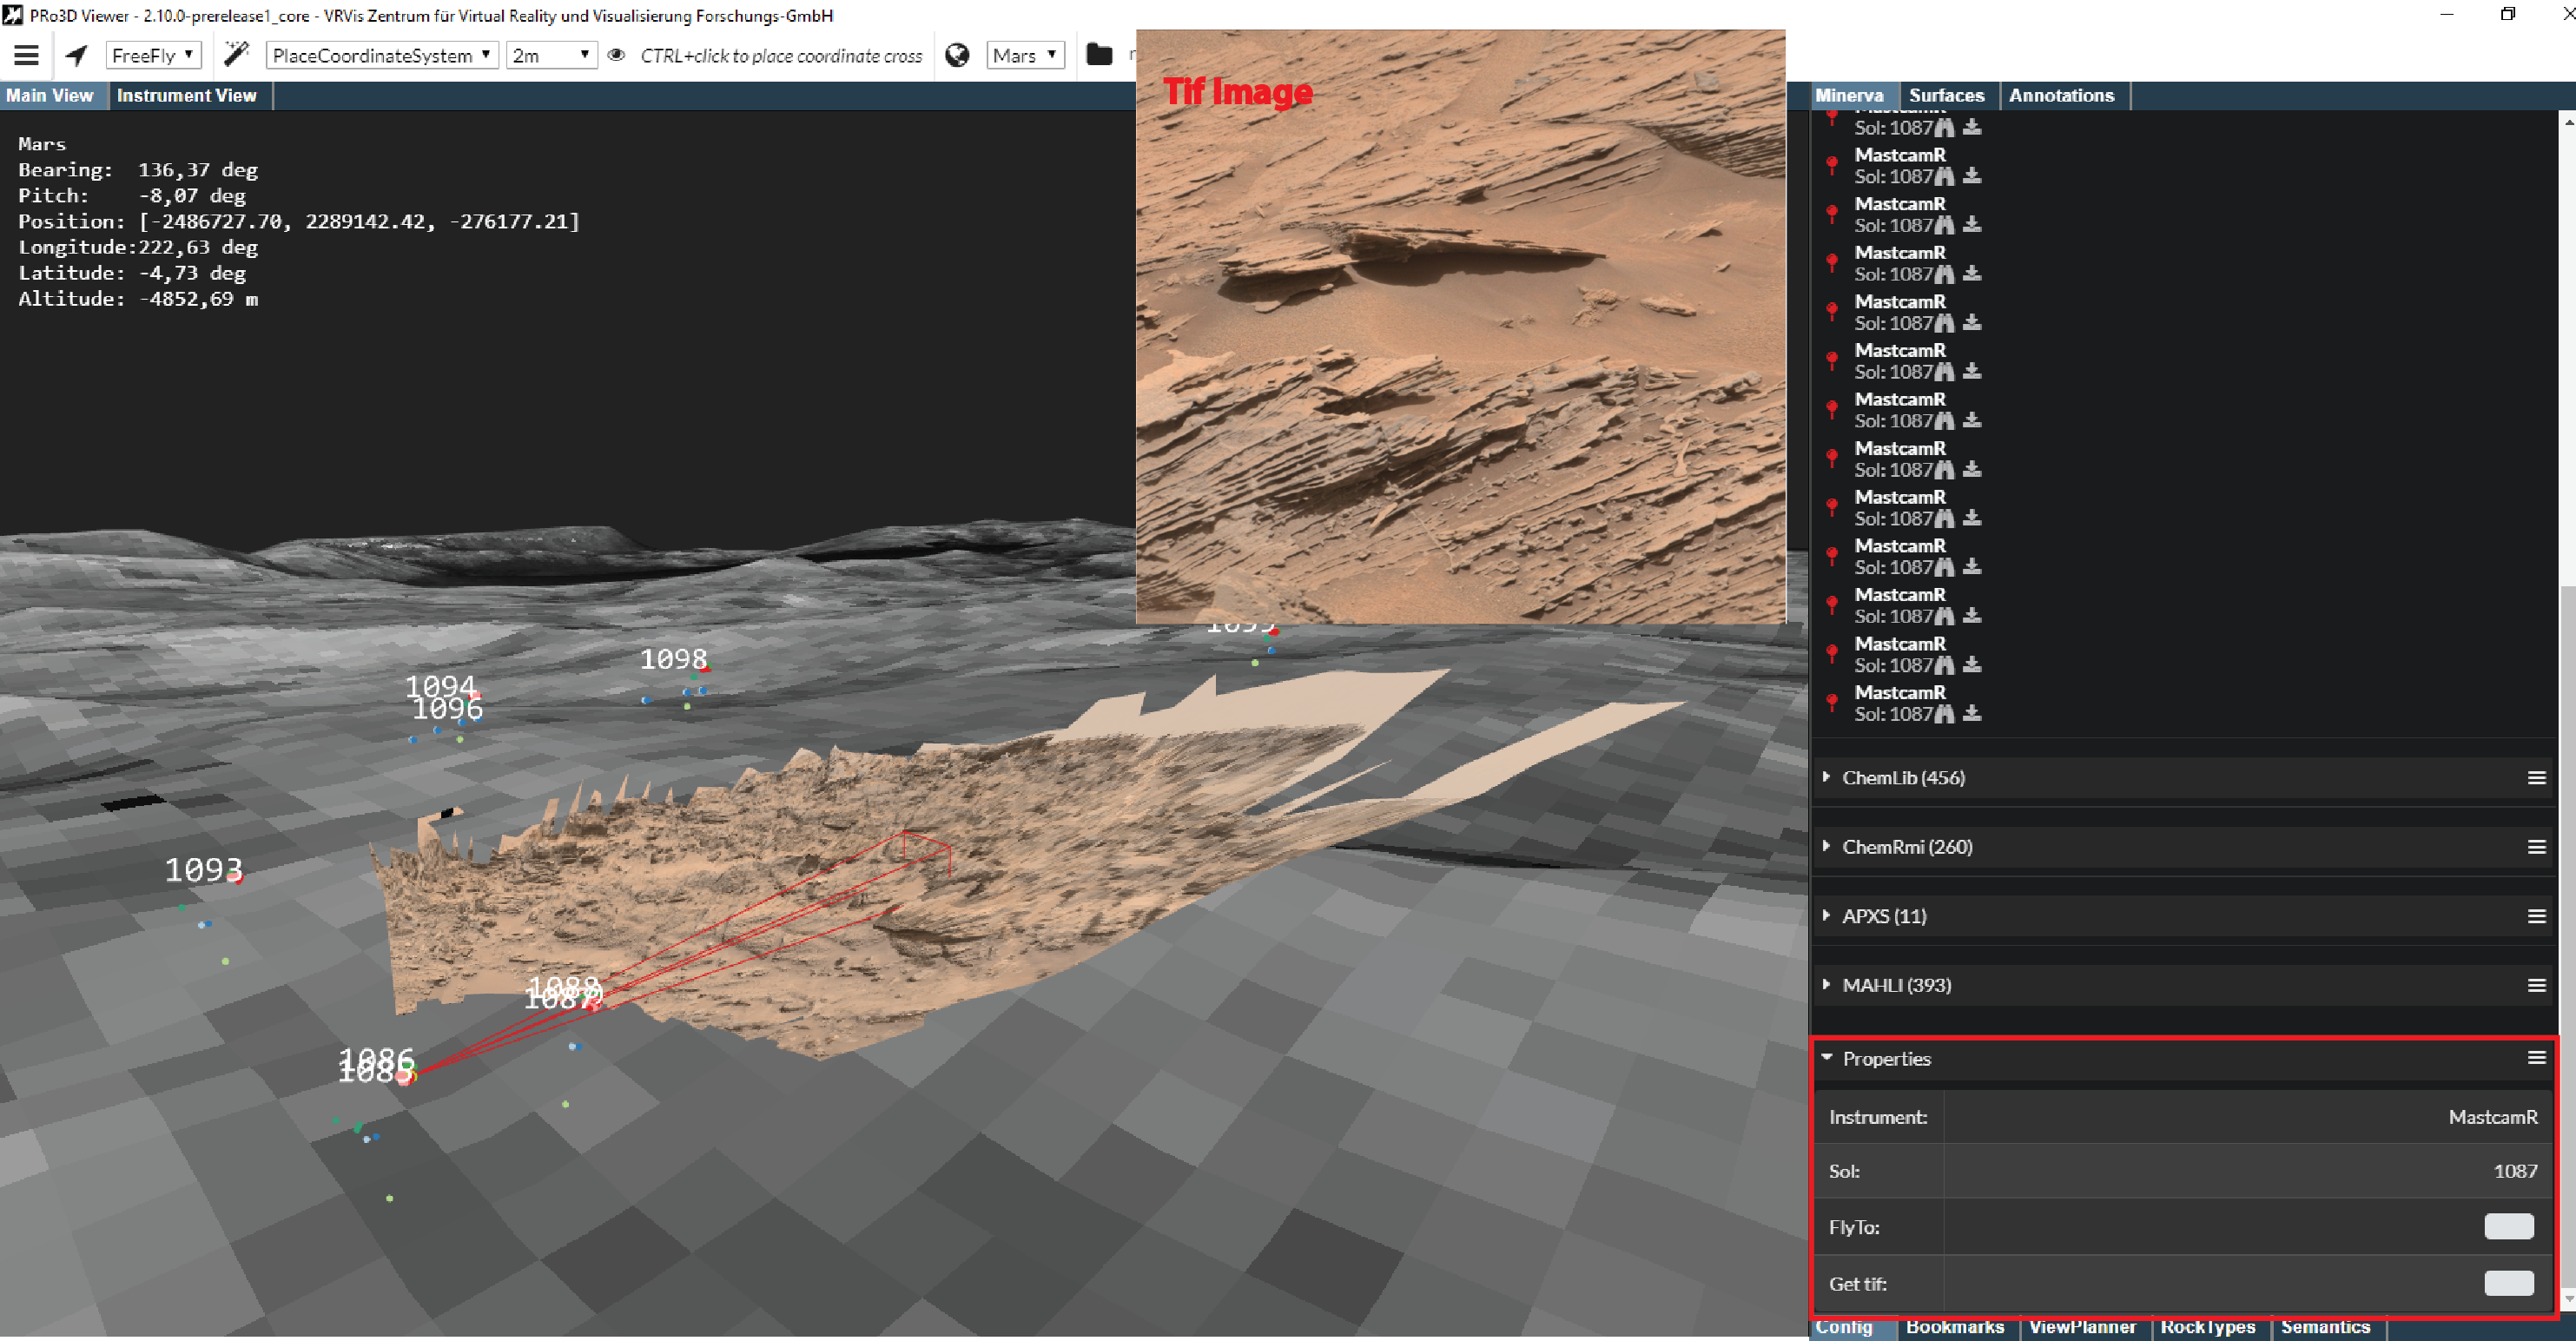
\includegraphics[width=1\textwidth]{pics/PropertiesAI.png}
				\caption[Product Properties]{The properties panel shows the sol number and provides interactions for the last selected product.}
				\label{fig:ProductProperties}
		 \end{figure}
		
The properties panel (Figure~\ref{fig:StartMinerva} D and Figure~\ref{fig:ProductProperties}) shows
\begin{itemize}
  \item \textbf{The Sol Number}
	\item \textbf{FlyTo}: A click on the button triggers a FlyTo animation.
	\item \textbf{GetTif}: Downloads the product's tif image. The image is stored in the \path{Release\netcoreapp2.0\MinervaData} folder.
\end{itemize}
of the last selected product.

%----------------------------------------------------------------------------------------
%	SubSection: Minerva Picking Actions
%----------------------------------------------------------------------------------------
\subsection{Picking Actions}
\label{sec:minervaPicking}

\begin{figure}[h]
				\centering
					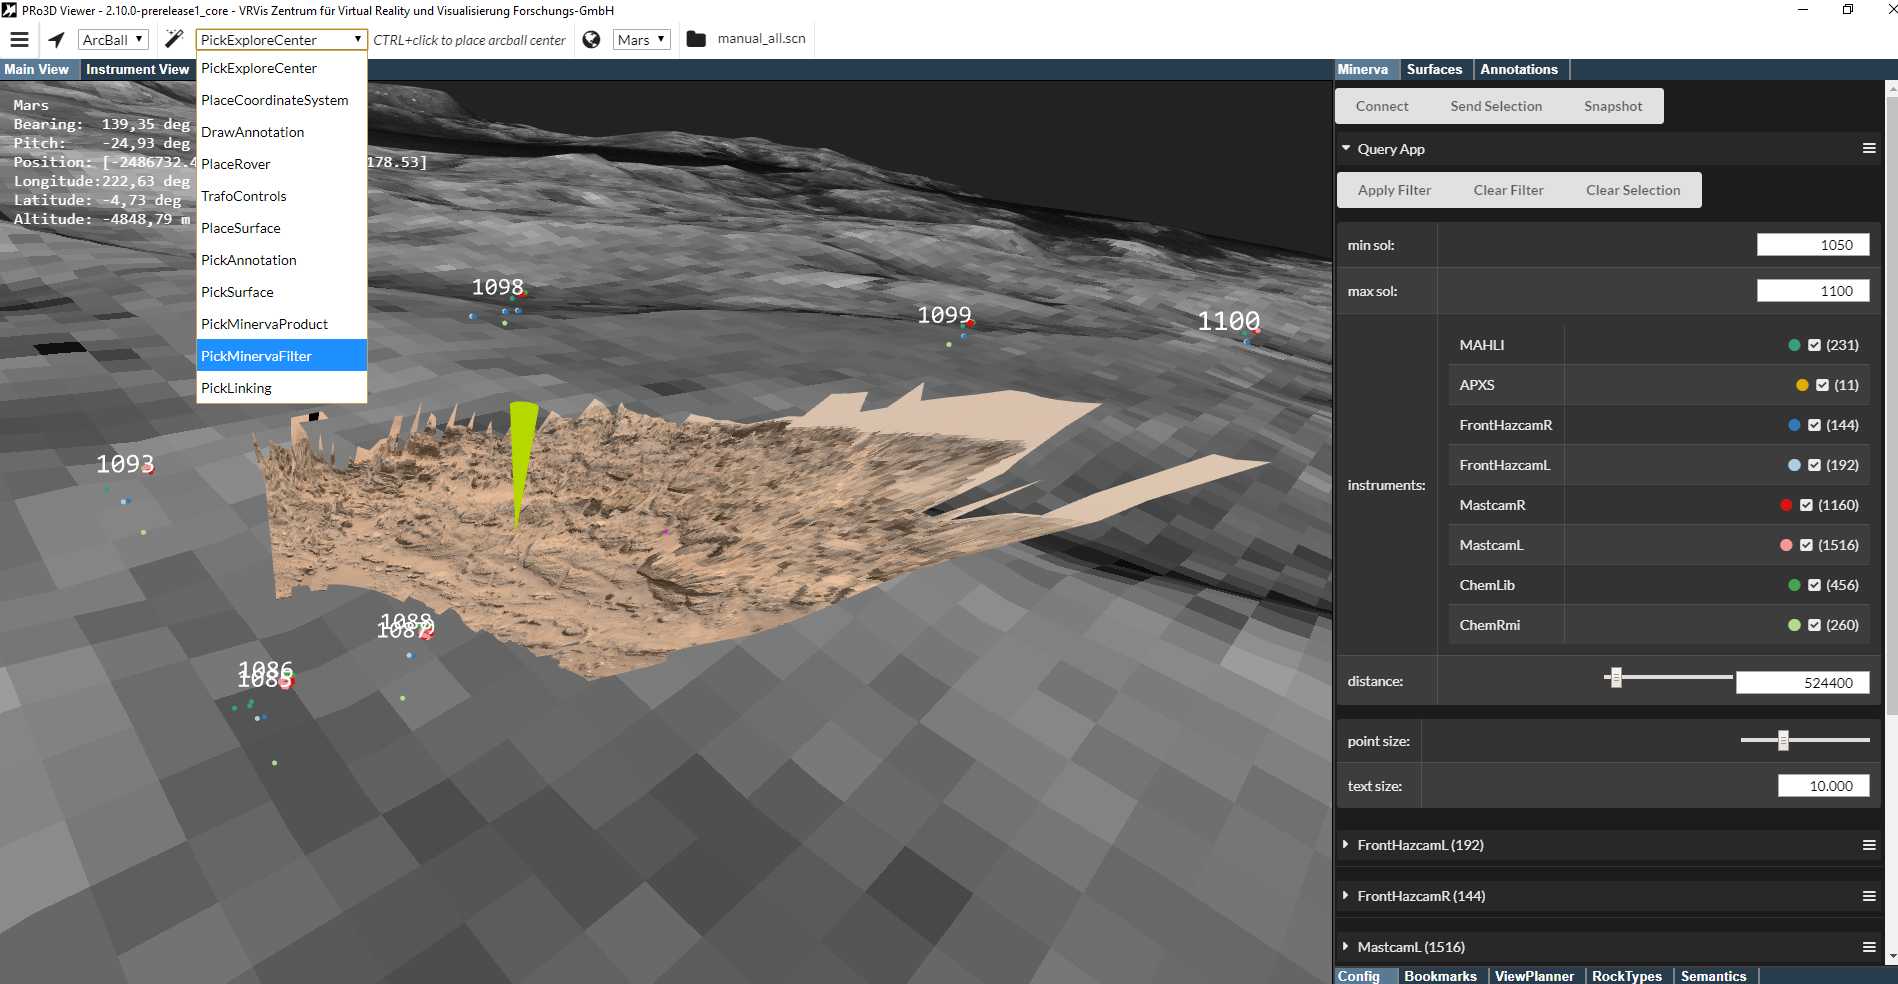
\includegraphics[width=1\textwidth]{pics/PickMinervaFilter.png}
				\caption[Pick Minerva Filter]{PickMinervaFilter}
				\label{fig:PickMinervaFilter}
		 \end{figure}
		
\begin{figure}[h]
				\centering
					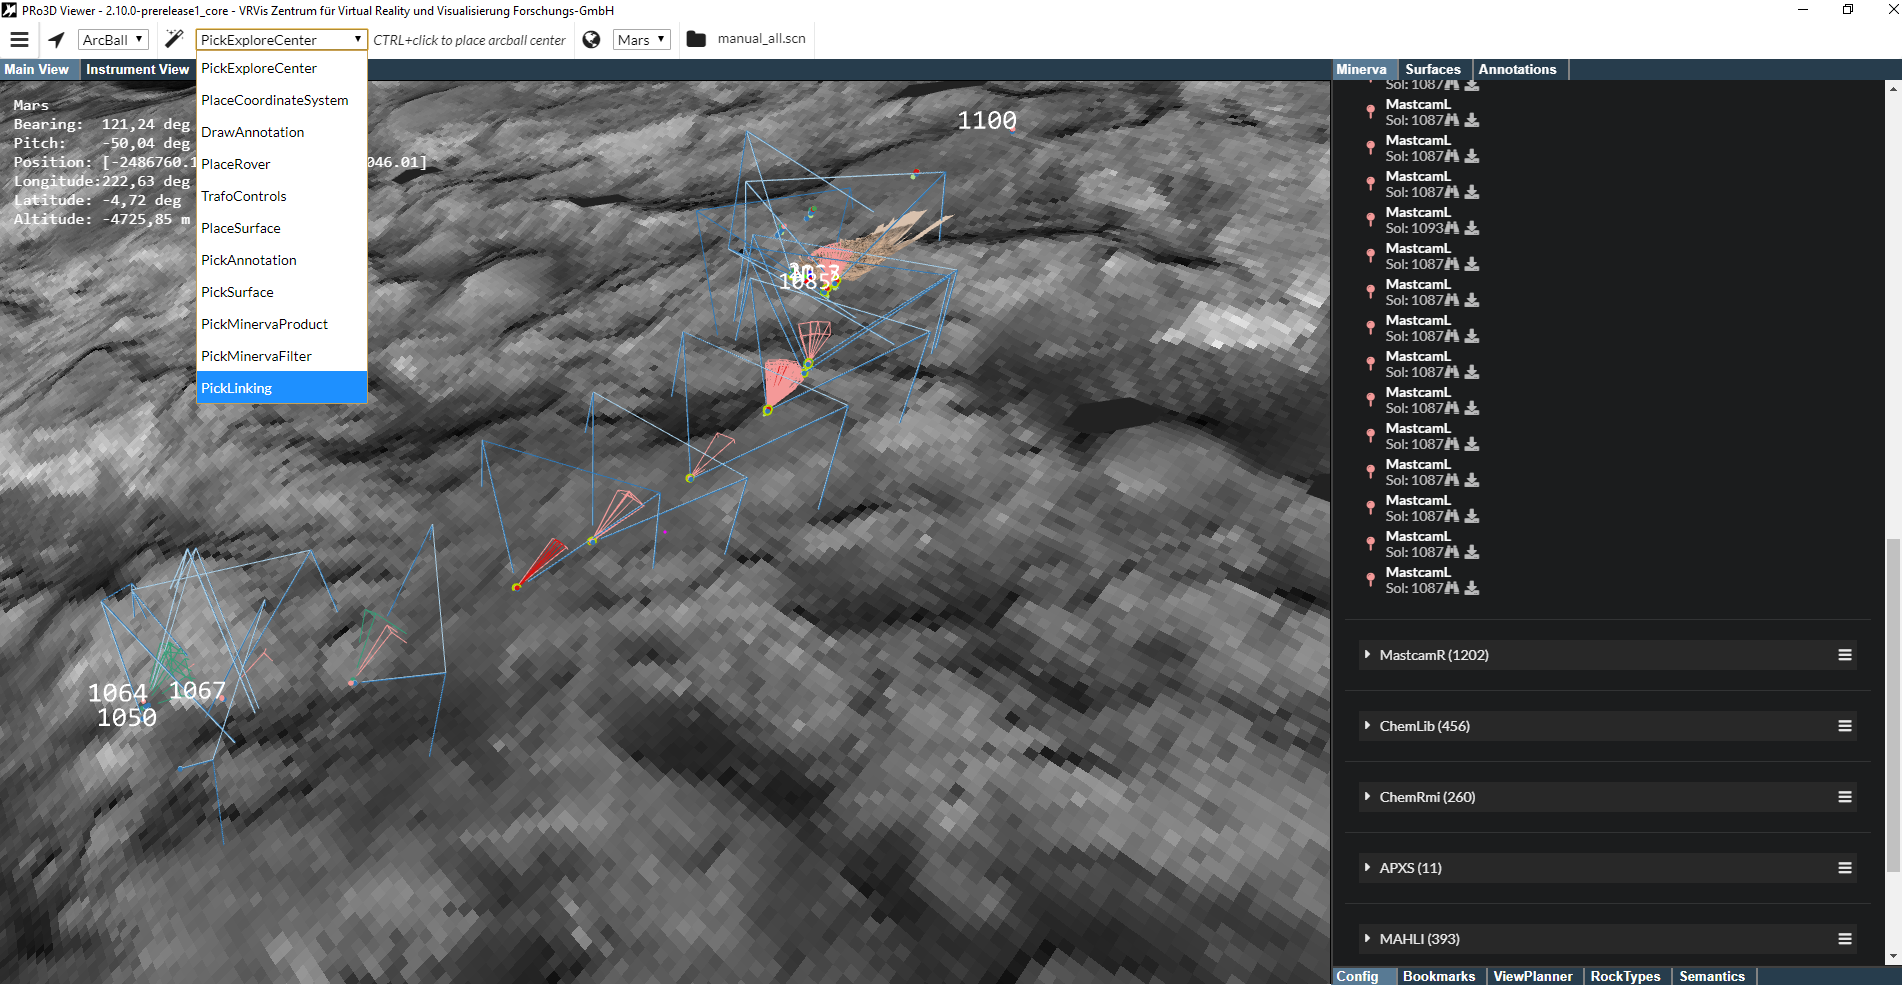
\includegraphics[width=1\textwidth]{pics/PickLinking1.png}
				\caption[Pick Linking]{PickLinking}
				\label{fig:PickLinking}
		 \end{figure}
		

There are three minerva picking actions in the picking actions drop down menu shown in Figure~\ref{fig:PickLinking}.
\\
\begin{itemize}
  \item \textbf{PickMinervaProduct}: You can set ``PickMinervaProduct'' in the actions menu to select a product in the Main View as described in Section~\ref{sec:selection}.
	\item \textbf{PickMinervaFilter}: Select ``PickMinervaFilter'' in the actions menu and press CTRL+LMB to pick a point on the surface. Then set a distance value with the distance slider in the Query App and click the ``ApplyFilter'' button. The products where the distance to the selected point is smaller than the selected distance in the Query App are shown (Figure~\ref{fig:PickMinervaFilter}).
	\item \textbf{PickLinking}: Select ``PickLinking'' in the actions menu and press CTRL+LMB to pick a point on the surface. All camera frustums of the products that captures the selected point are shown (Figure~\ref{fig:PickLinking}).
\end{itemize}


%----------------------------------------------------------------------------------------
%	END OF DOCUMENT
%----------------------------------------------------------------------------------------
\end{document}

